In this section, we study the stability of the presented method for the linear Dahlquist equation $u' = -\lambda u$ or $u' = -\lambda_I u - \lambda_E u$ for IMEX methods. All methods can be rewritten as $u_{n+1} = R(z)u_n$ or $u_{n+1}= R(z_I,z_E)$ being $R$ stability functions and $z,z_I,z_E\in \mathbb C$. 
We will study the stability regions $\lbrace |R|\leq 1\rbrace \subset \mathbb C$ for the explicit and implicit ADER/DeC, while for the IMEX schemes we consider different approaches. 
We will use equispaced (eq) or Gauss-Lobatto (GLB) nodes as quadrature nodes.
We will numerically compute the stability regions obtained from the stability functions of ADER/DeC that are defined through their Butcher tableaux, see \cite{hairer1987solving}.
In detail, we compute on $200\times 200$ grid points with an offset of $+0.01$ from the origin for both axes to avoid singularities. 
The plot bounds are dependent on the type of scheme and their stability regions.
We decreased the offset in Figures~\ref{fig: ODE_minor_instabilitys} to a fraction of $10^{-2}$ of the largest real value displayed when zooming on small areas.

%All of the following pictures have been obtained by plugging the above described Butcher tableaux into the stability functions, using property \eqref{eq:ImExStabilityFunction} and evaluating them numerically.\\
%While the explicit cases have already been investigated in \cite{Han_Veiga_2021}, we will investigate the implicit stability regions for the first time at this point. 
%A slight extension to these results can be found in the appendix.
To distinguish the different orders, we apply different colors and line styles to the outer and inner bounds according to the legend that are plot next to each stability region plot.
%in figure~\ref{fig: legend_standard}.
%\begin{figure}[!h]
%	\centering
%		\begin{minipage}[t]{0.4\textwidth}\centering
%			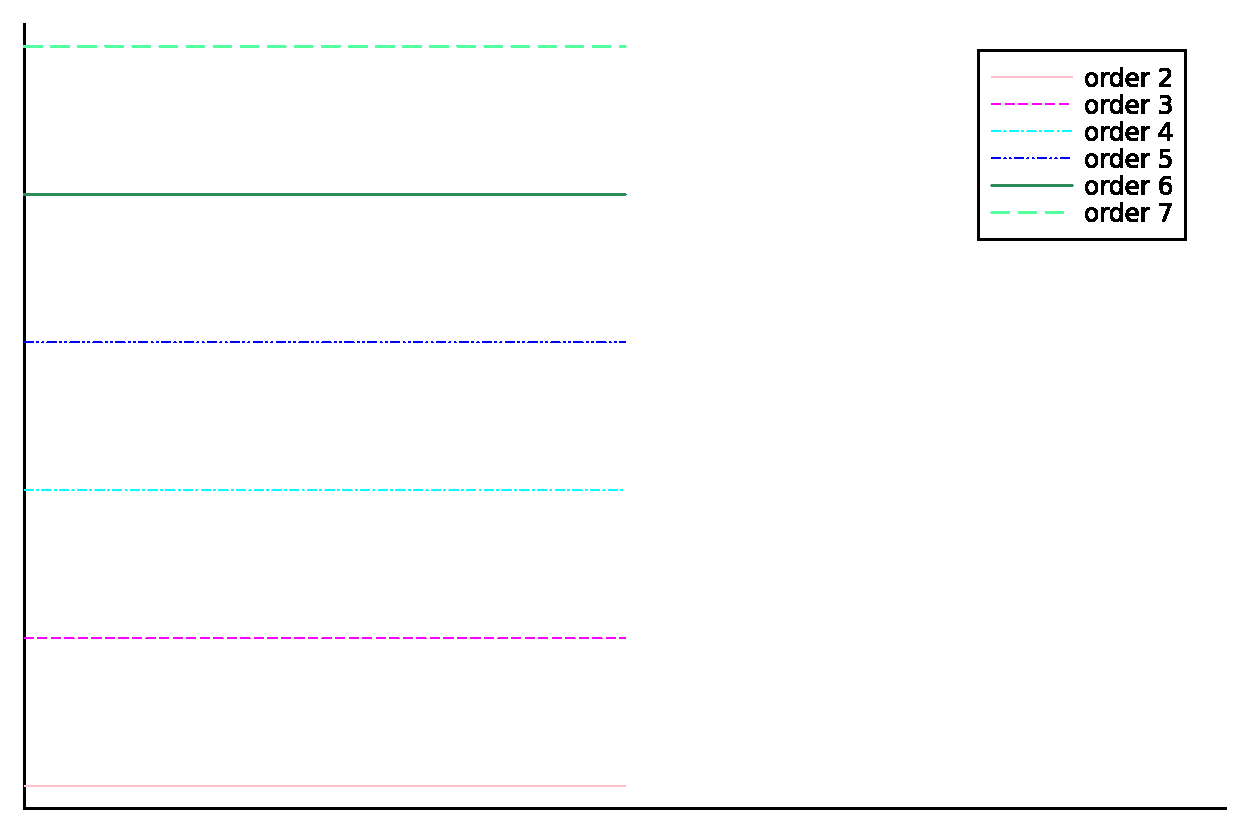
\includegraphics[height=0.4\textwidth, trim={469 280 30 23}, clip]{pdf/odepics/colors_a-d_new_2-7.pdf}
%			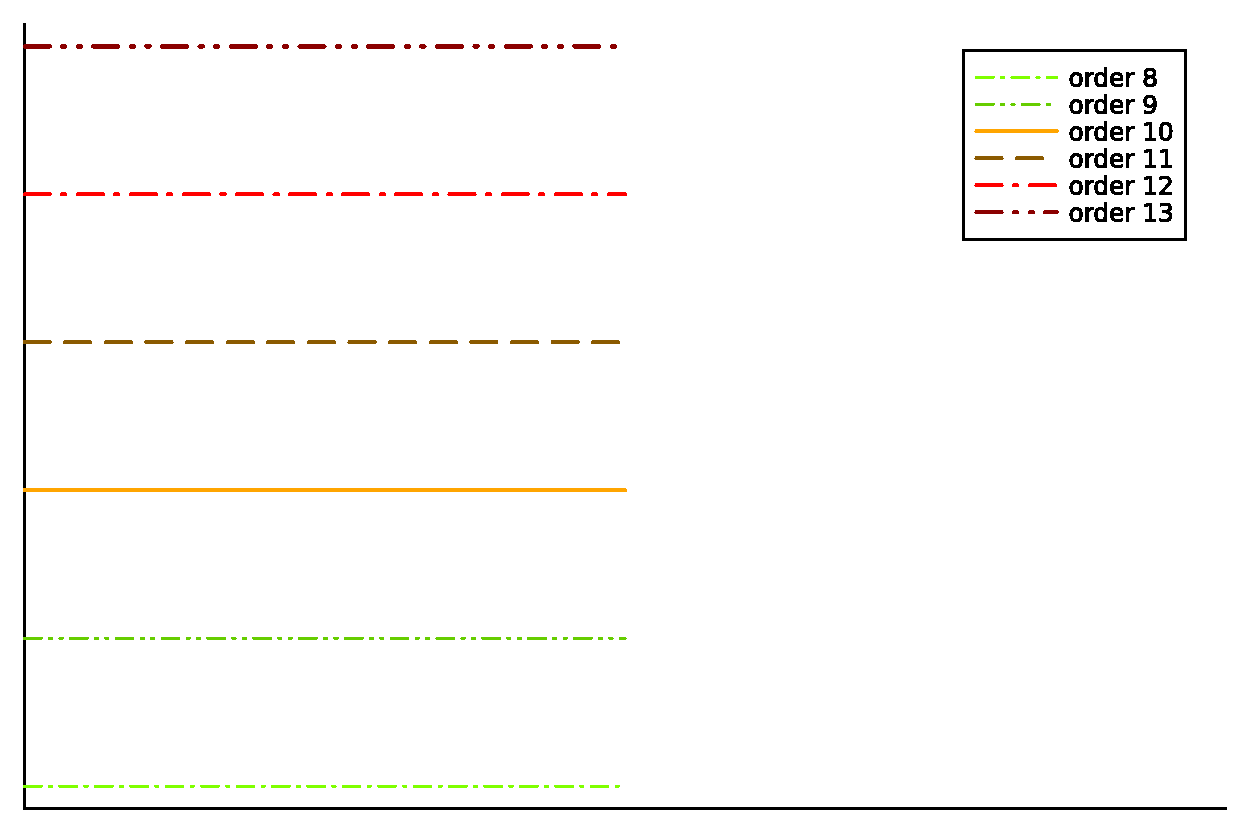
\includegraphics[height=0.4\textwidth, trim={461 280 30 23}, clip]{pdf/odepics/colors_a-d_new_8-13.pdf}
%		\end{minipage}
%		\caption{Legend for the classic RK and the IMEX stability regions}
%	\label{fig: legend_standard}
%\end{figure}
\subsection{Explicit schemes}
\subsection{Stability analysis of explicit schemes}\label{sec:stability_explicit}
In figure~\ref{fig: ODEEXADERDeCeq}, we show the results obtained in \cite{Han_Veiga_2021}, extended up to order 13. It was pointed out, that the regions of the explicit ADER and DeC coincide and that they are independent of the chosen interpolation nodes. Here, we just display them once. We can highlight the growth of stability by increasing the order of the respective method. 
\begin{figure}[!h]
	\centering
	\begin{minipage}[t]{0.45\textwidth}
		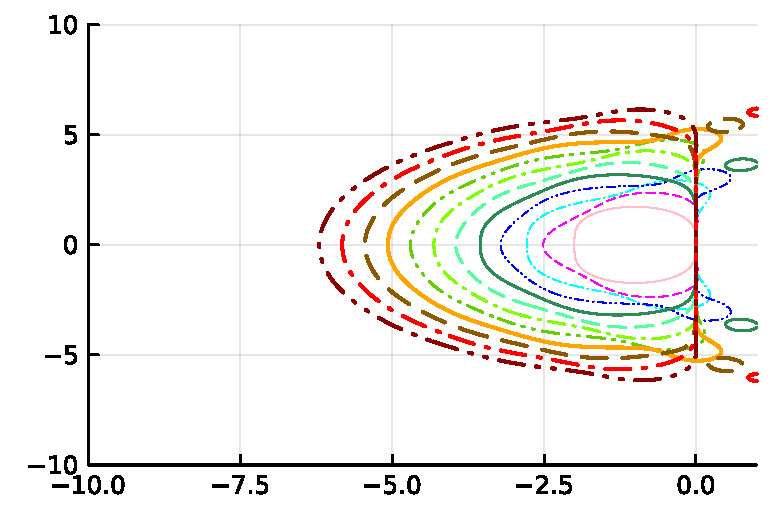
\includegraphics[width=\textwidth,trim={0 0 0 22}, clip]{pdf/odepics/DeC_GLB_ord13.pdf}
	\end{minipage}
	\caption{Stability regions for the explicit ADER and DeC methods with GLB or equispaced nodes for orders 2 to 13.}
	\label{fig: ODEEXADERDeCeq}
\end{figure}

Furthermore, we want to take a look at the explicit sDeC, whose stability regions can be observed in figure~\ref{fig: ODEEXsDeC}. 
This method differs not only from the ADER and DeC, but also from sDeC with different nodes. The qualitative shape is still similar to the others, but it is just remarkable that the sDeC methods with equispaced interpolation points have respectively larger stability regions.

\begin{figure}
	\centering
	\begin{minipage}[t]{0.45\textwidth}
		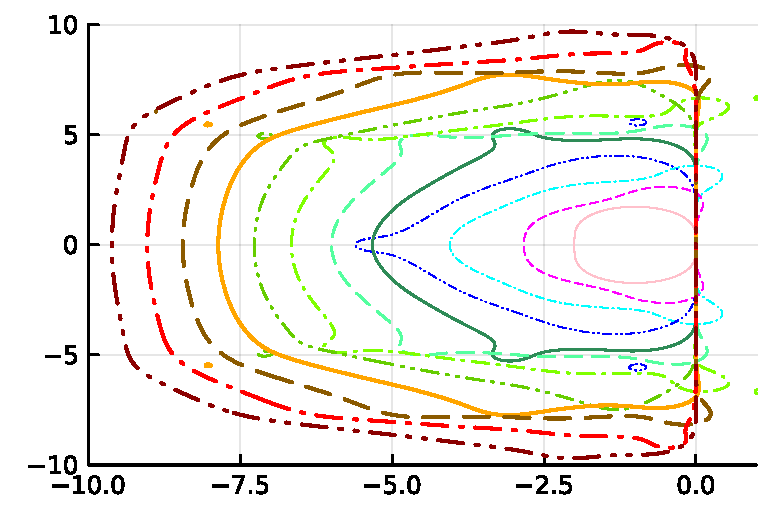
\includegraphics[width=\textwidth]{pdf/odepics/sDeC_eq_ord13.pdf}
	\end{minipage}
	\begin{minipage}[t]{0.45\textwidth}
		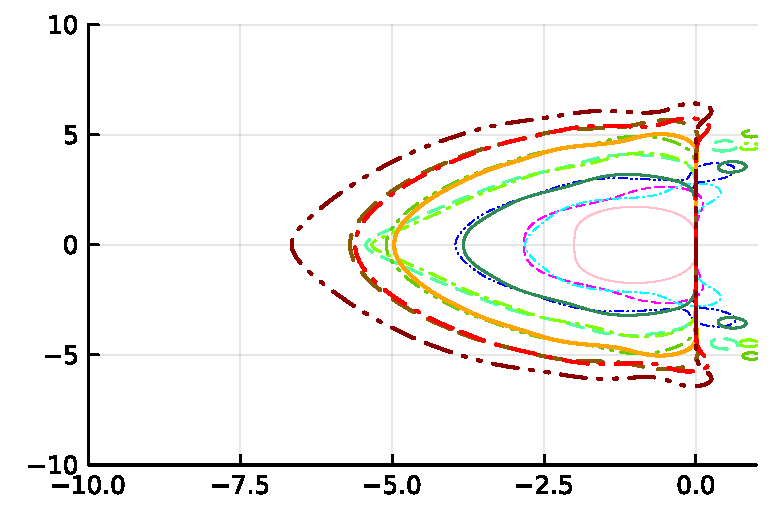
\includegraphics[width=\textwidth]{pdf/odepics/sDeC_GLB_ord13.pdf}
	\end{minipage}
	\caption{sDeC for orders 2 to 13.}
	\label{fig: ODEEXsDeC}
\end{figure}
\subsection{Implicit schemes}
In the following, we plot the contour lines of the bounds of the stability regions of various implicit methods. We start from ImDeC and ImADER schemes with equispaced nodes and GLB nodes in Figure~\ref{fig: ODEIMDeCADER}. 
Clearly, all these stability regions are unbounded, but they are not all A-stable, as we will see soon. Moreover, we can observe a great variability changing the scheme or the nodes, in opposition to the explicit case \cite{Han_Veiga_2021}. In most of the cases, ImADER have larger stability regions than ImDeC.
%We already see a different behavior in stability, contrary to the explicit counterparts. 
%We also observe a slightly different behavior while changing the interpolation nodes to Gauss-Lobatto points in figure~\ref{fig: ODEIMDeCADERGLB}. Nevertheless, all the results coincide with what expected from implicit Runge-Kutta schemes and all the methods seem to be A-stable. Furthermore, the stability regions of the ImADER differ to the ImDeC for both types of nodes, differently from the explicit case \cite{Han_Veiga_2021}.  
\begin{figure}
	\centering
	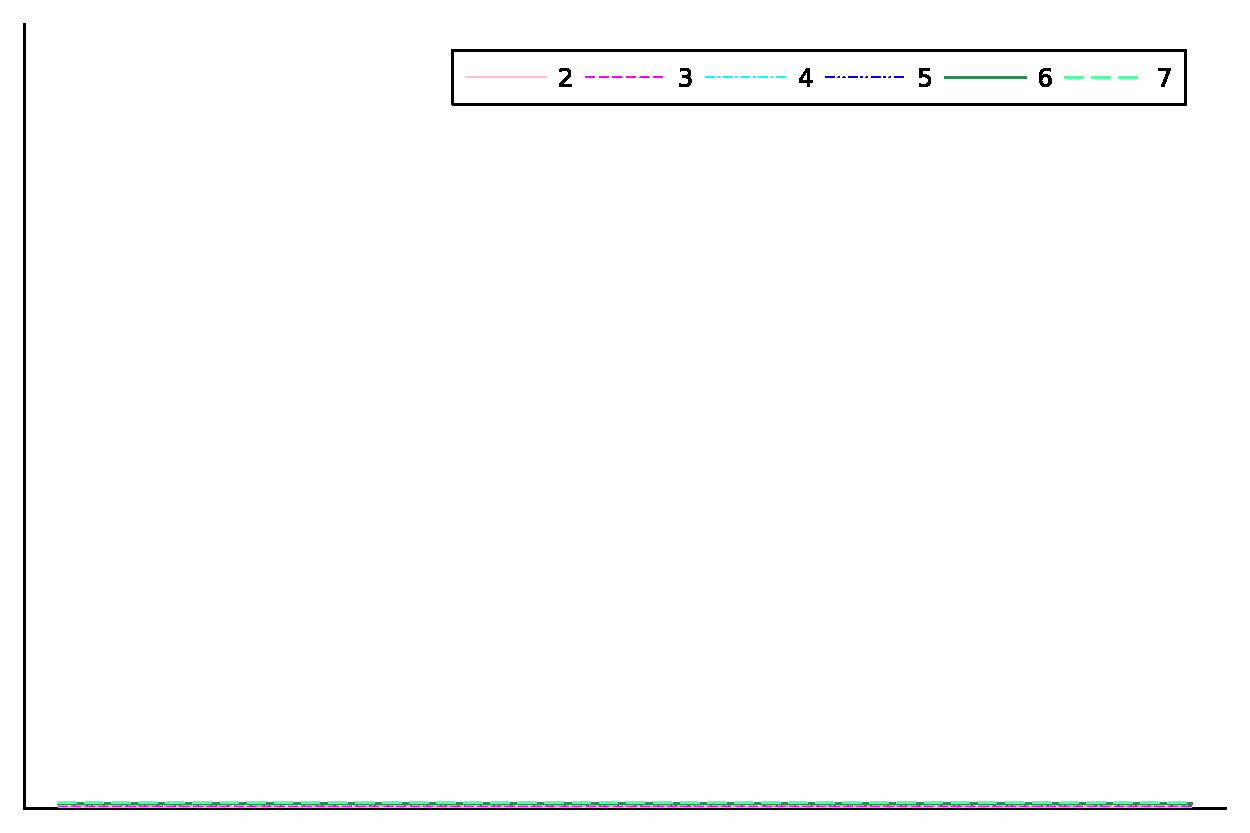
\includegraphics[width=0.465\textwidth,trim={215 340 32 22}, clip]{pdf/odepics/colors_a-d_new_horiz_2-7_no_order.pdf}\!\!
	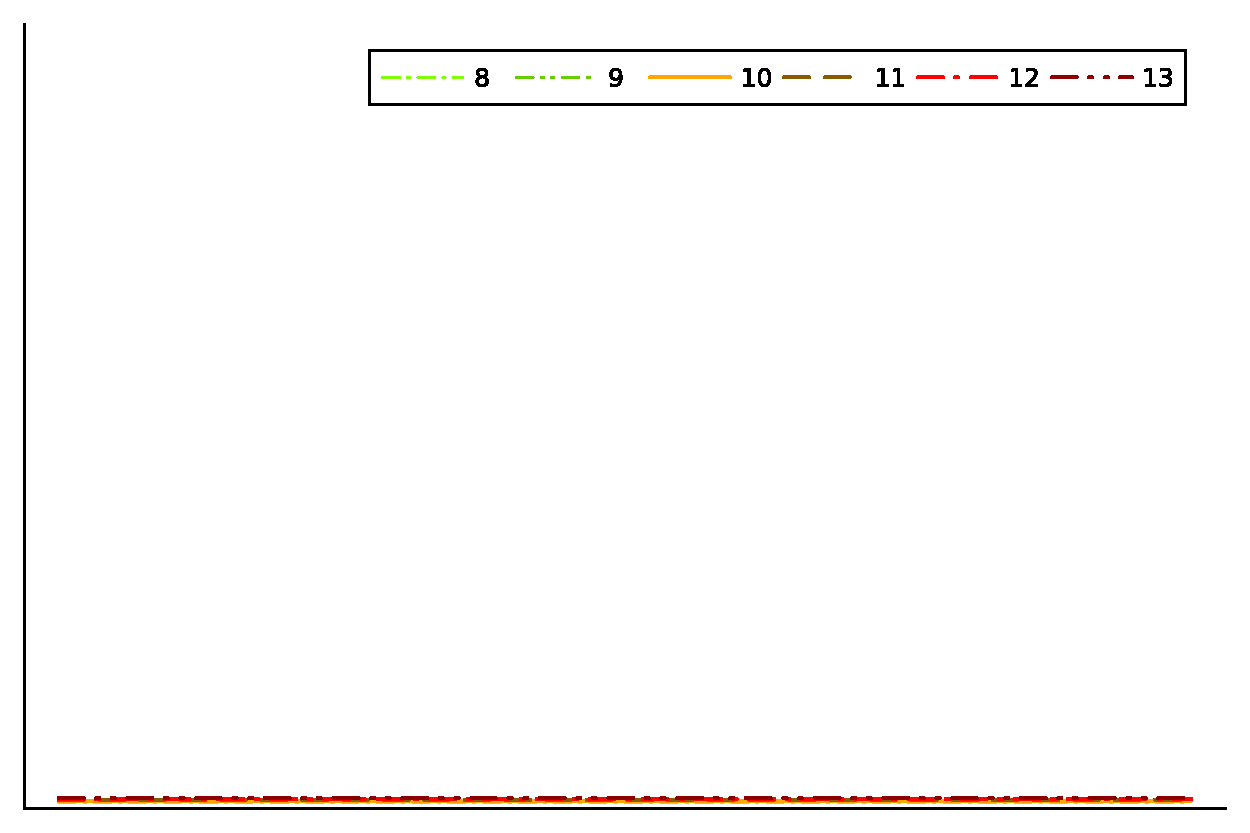
\includegraphics[width=0.515\textwidth,trim={178 340 30 22}, clip]{pdf/odepics/colors_a-d_new_horiz_8-13_no_order.pdf}\\
	\begin{minipage}[t]{0.32\textwidth}
		\centering
		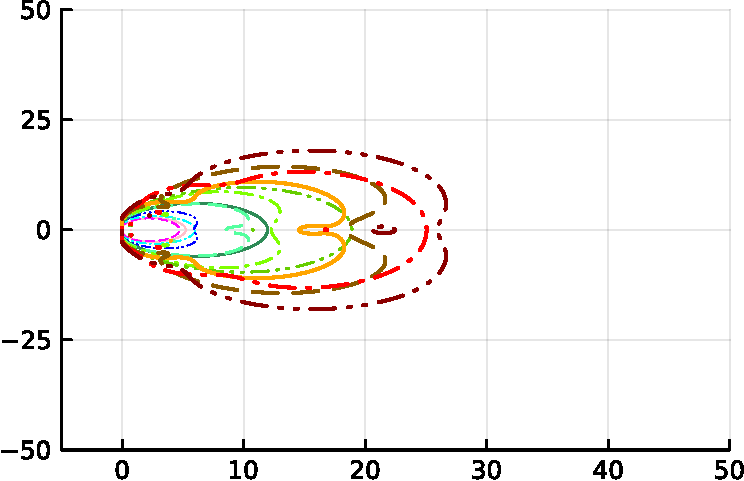
\includegraphics[width=\textwidth, trim={0 0 0 22}, clip]{pdf/odepics/IMDeC_eq_ord13-crop.pdf}\\
		ImDeC eq
	\end{minipage}
	\begin{minipage}[t]{0.32\textwidth}
		\centering
	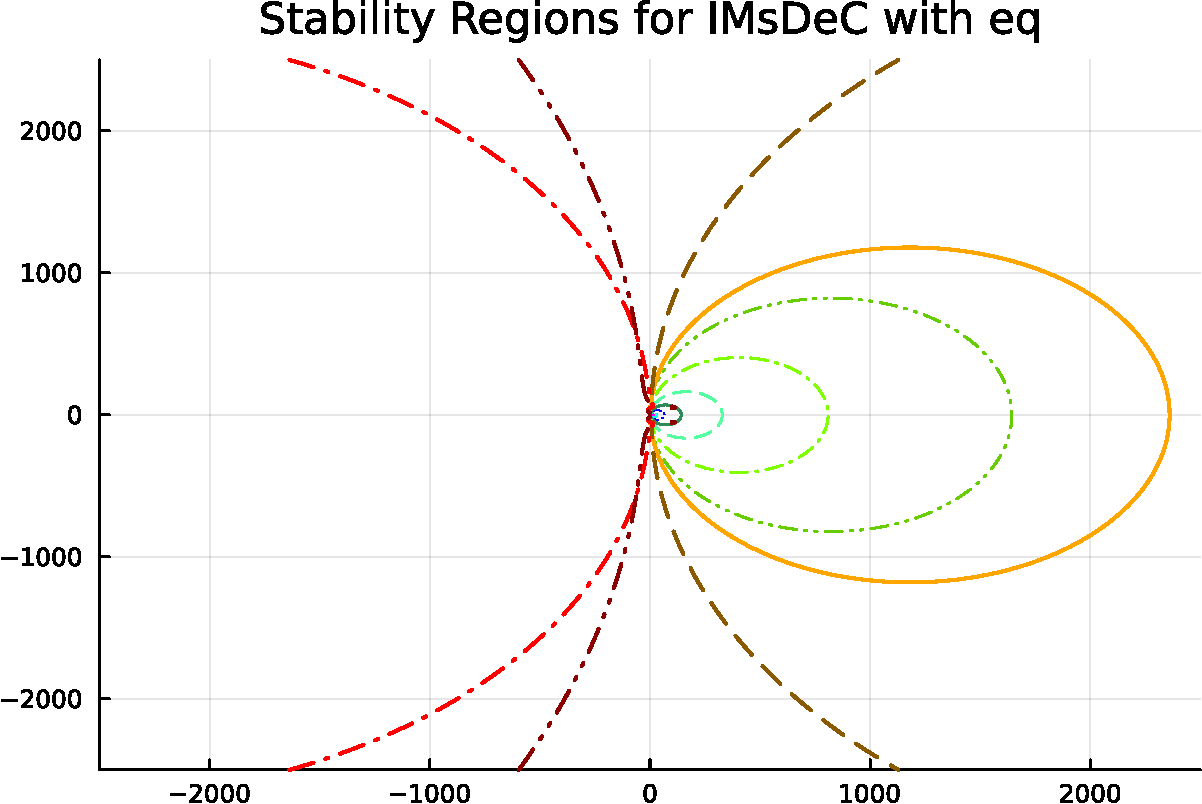
\includegraphics[width=\textwidth, trim={0 0 0 22}, clip]{pdf/odepics/IMsDeC_eq_ord13-crop.pdf}\\
	ImsDeC eq
	\end{minipage}
	\begin{minipage}[t]{0.32\textwidth}
		\centering
		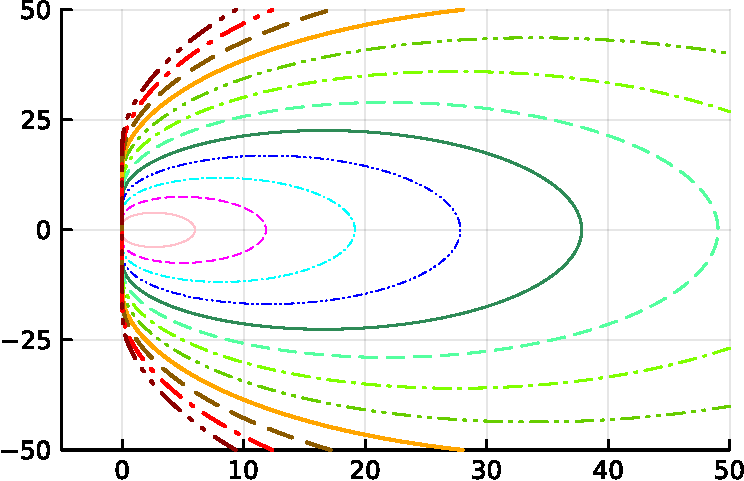
\includegraphics[width=\textwidth, trim={0 0 0 22}, clip]{pdf/odepics/IMADER_eq_ord13-crop.pdf}\\
		ImADER eq
	\end{minipage}\\
%	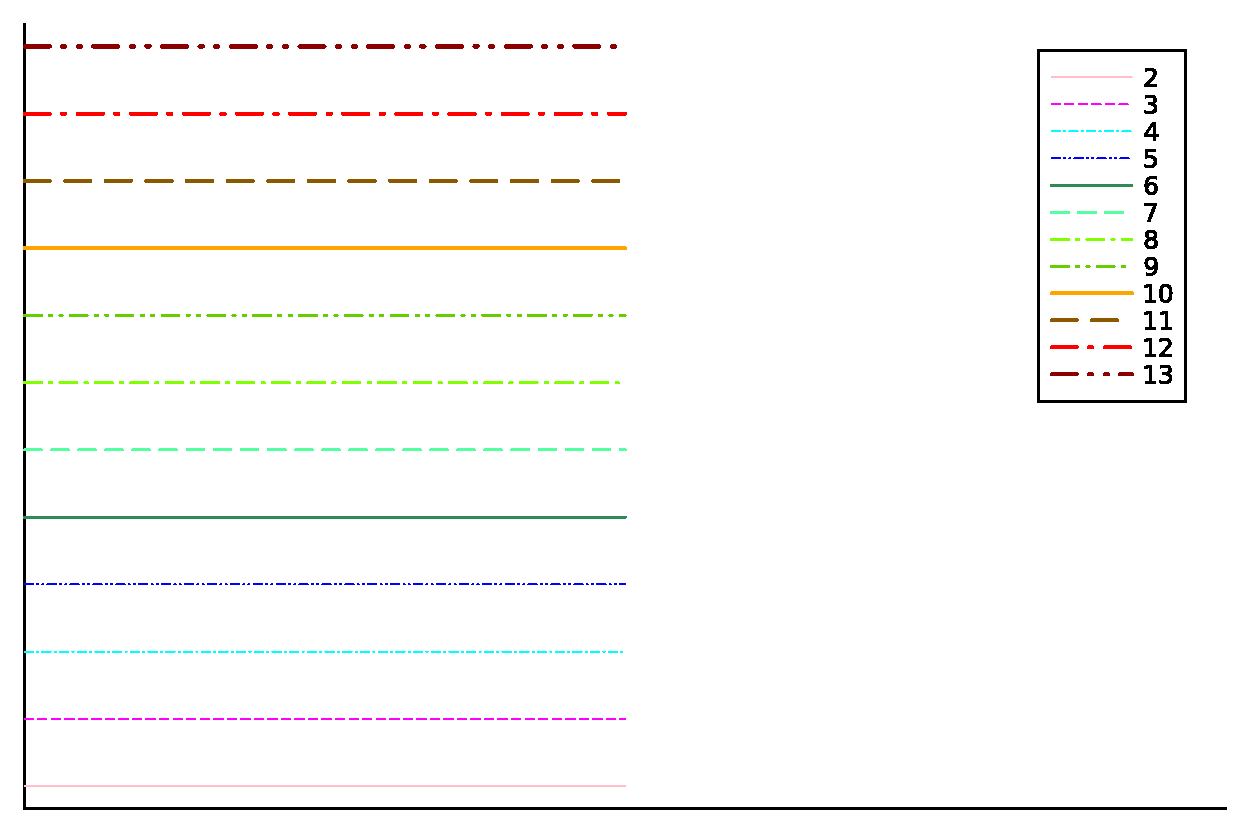
\includegraphics[width=0.08\textwidth, trim={491 140 30 23}, clip]{pdf/odepics/colors_a-d_new_2-13_no_order.pdf}\\
	\begin{minipage}[t]{0.32\textwidth}
		\centering
		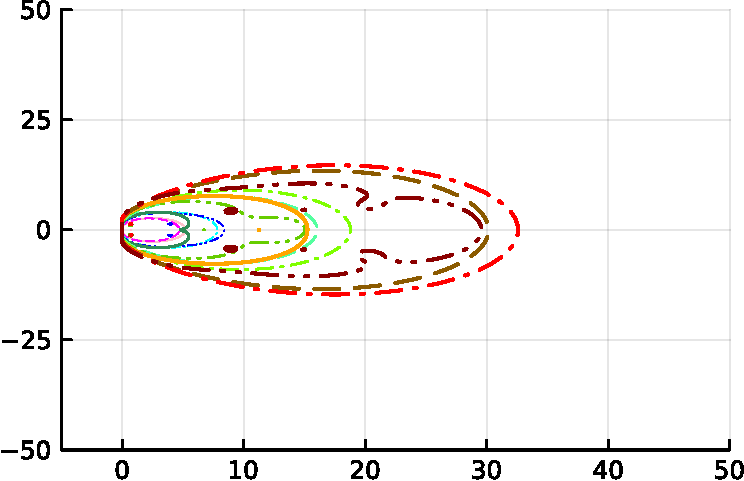
\includegraphics[width=\textwidth, trim={0 0 0 22}, clip]{pdf/odepics/IMDeC_GLB_ord13-crop.pdf}\\
		ImDeC GLB
	\end{minipage}
	\begin{minipage}[t]{0.32\textwidth}
		\centering
	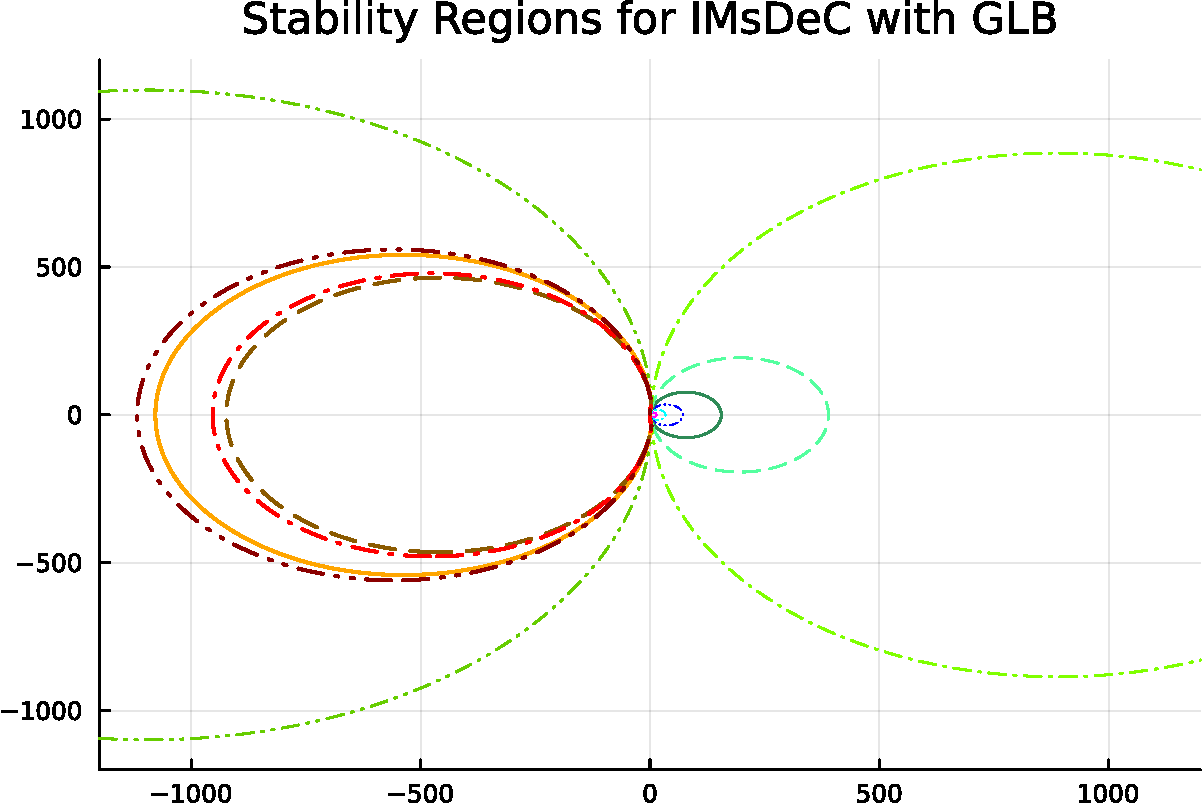
\includegraphics[width=\textwidth, trim={0 0 0 22}, clip]{pdf/odepics/IMsDeC_GLB_ord13-crop.pdf}\\
	ImsDeC GLB
	\end{minipage}
	\begin{minipage}[t]{0.32\textwidth}
		\centering
		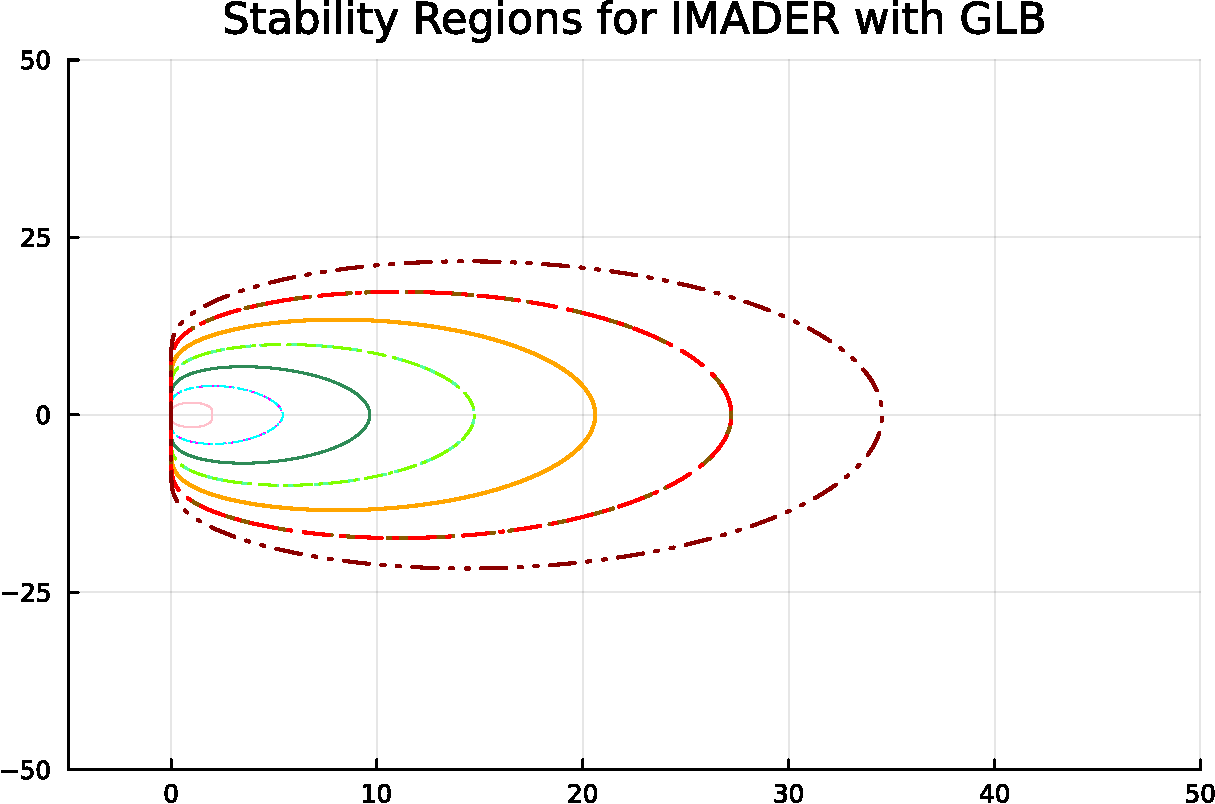
\includegraphics[width=\textwidth, trim={0 0 0 22}, clip]{pdf/odepics/IMADER_GLB_ord13-crop.pdf}\\
		ImADER GLB
	\end{minipage}
%	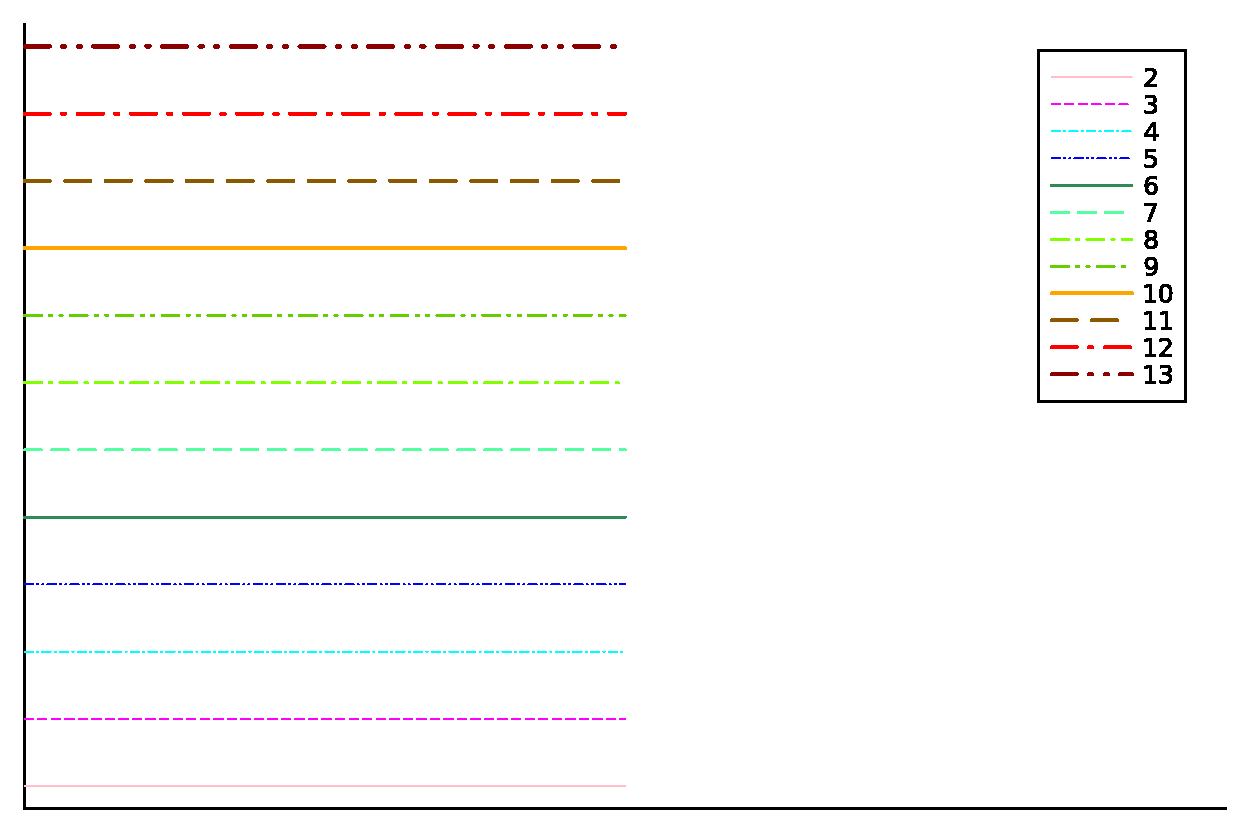
\includegraphics[width=0.08\textwidth, trim={491 140 30 23}, clip]{pdf/odepics/colors_a-d_new_2-13_no_order.pdf}
	\caption{Implicit DeC (left), sDeC (center) and ADER (right) with equispaced (top) and Gauss-Lobatto (bottom) nodes for orders 2 to 13}
	\label{fig: ODEIMDeCADER}
\end{figure}
%\begin{figure}
%	\centering
%	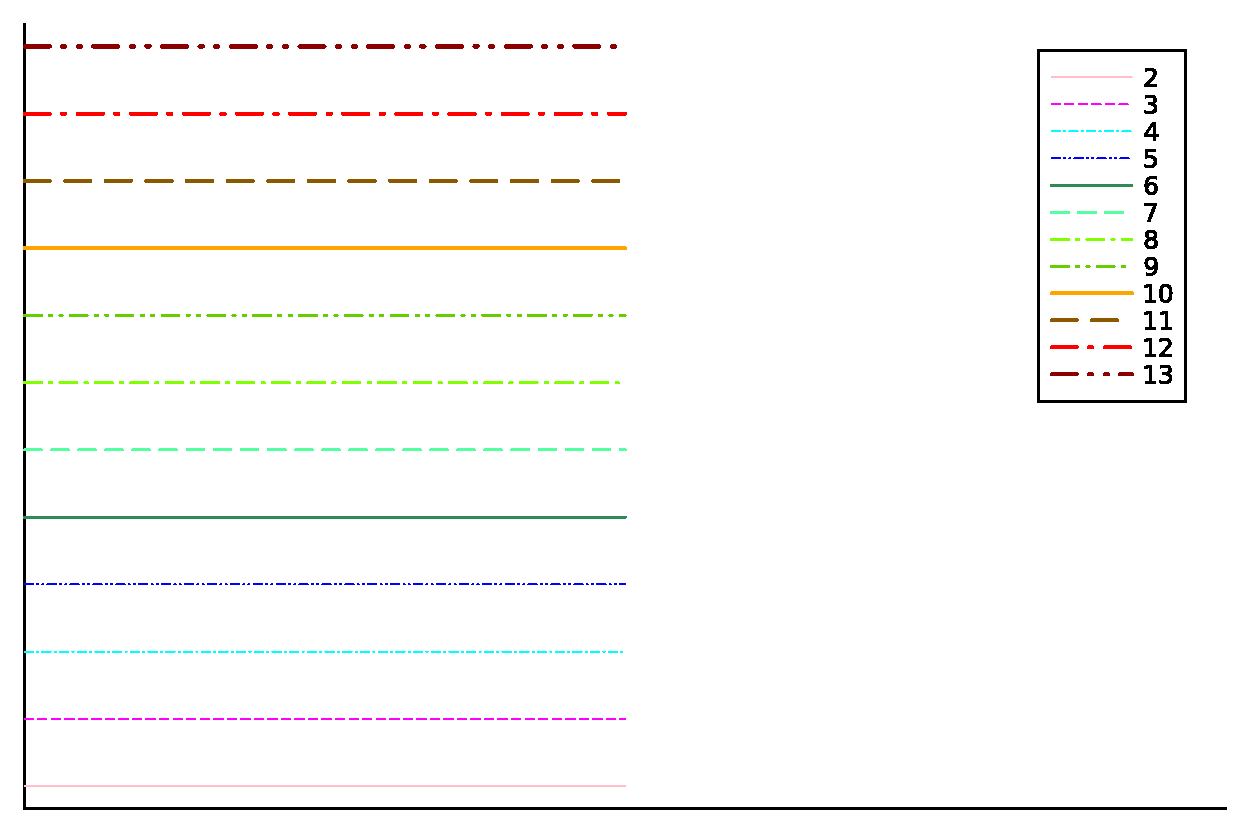
\includegraphics[width=0.08\textwidth, trim={491 180 30 23}, clip]{pdf/odepics/colors_a-d_new_2-13_no_order.pdf}
%	\caption{Implicit sDeC for orders 2 to 13}
%	\label{fig: ODEIMsDeC}
%\end{figure}

\begin{figure}
	\centering
	\begin{minipage}[t]{0.45\textwidth}
		\centering
		\includegraphics[width=\textwidth, trim={0 0 0 22}, clip]{pdf/odepics/ImsDeC_eq_ord20-crop.pdf}\\
		ImsDeC eq
	\end{minipage}
	\begin{minipage}[t]{0.45\textwidth}
		\centering
		\includegraphics[width=\textwidth, trim={0 0 0 22}, clip]{pdf/odepics/ImsDeC_GLB_ord20-crop.pdf}\\
		ImsDeC GLB
	\end{minipage}
	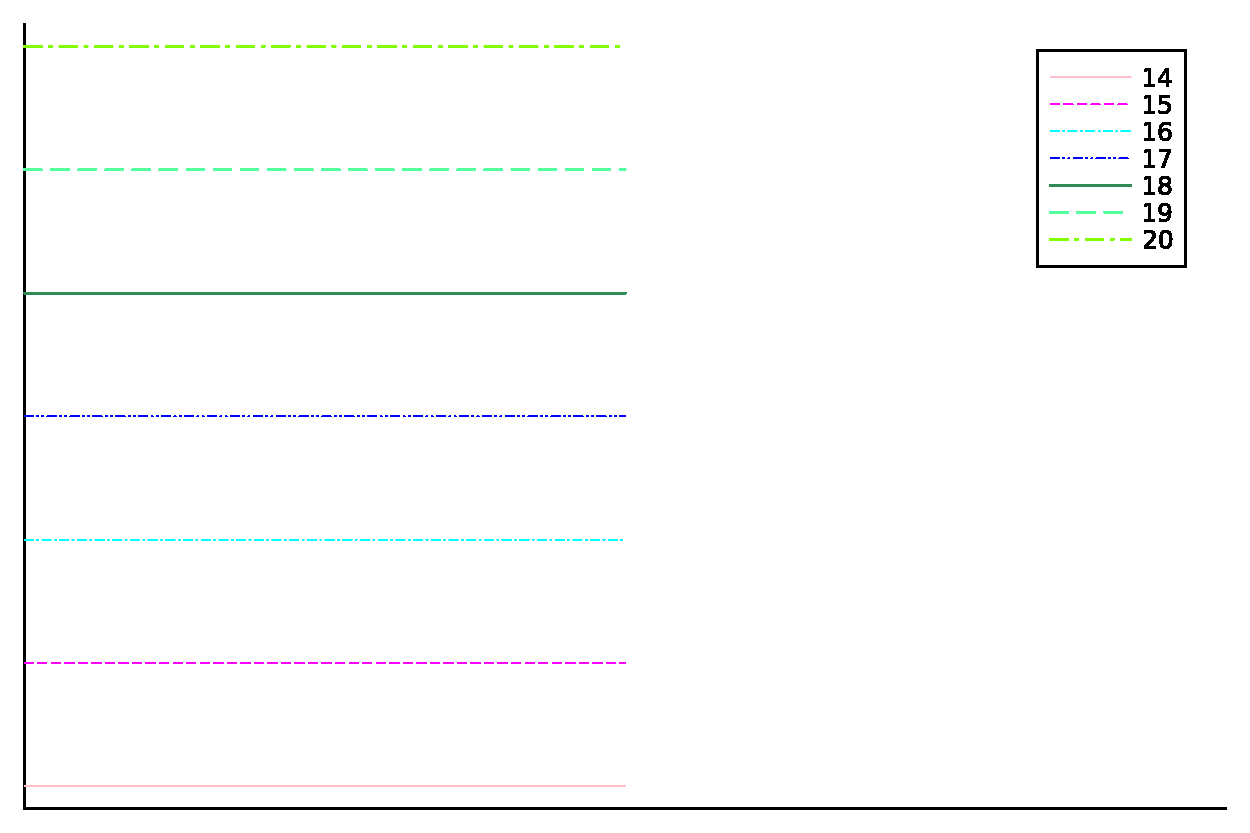
\includegraphics[width=0.08\textwidth, trim={491 180 30 23}, clip]{pdf/odepics/colors_a-d_new_14-20_no_order.pdf}
	\caption{Implicit sDeC for orders 14 to 20}
	\label{fig: exaImsDeC_high}
\end{figure}
The stability regions for the implicit sDeC (ImsDeC) are also shown in Figure~\ref{fig: ODEIMDeCADER} and, surprisingly, do not behave like the other methods. 
Up to a certain order (i.e. sDeC8 with Gauss-Lobatto and sDeC11 with equispaced nodes), the stability regions are unbounded and \textit{seem} A-stable, but for higher orders, we lose this property, obtaining large, but finite, stability regions. 
This behavior is not uniform and, at certain orders, the stability region will be unbounded again, as for example shown in Figure~\ref{fig: exaImsDeC_high} for very high order ImsDeC. 

%A legend for these plots can be found in figure~\ref{fig: legend_high_order}.
%\begin{figure}[!h]
%	\centering
%	\begin{minipage}[t]{0.18\textwidth}
%		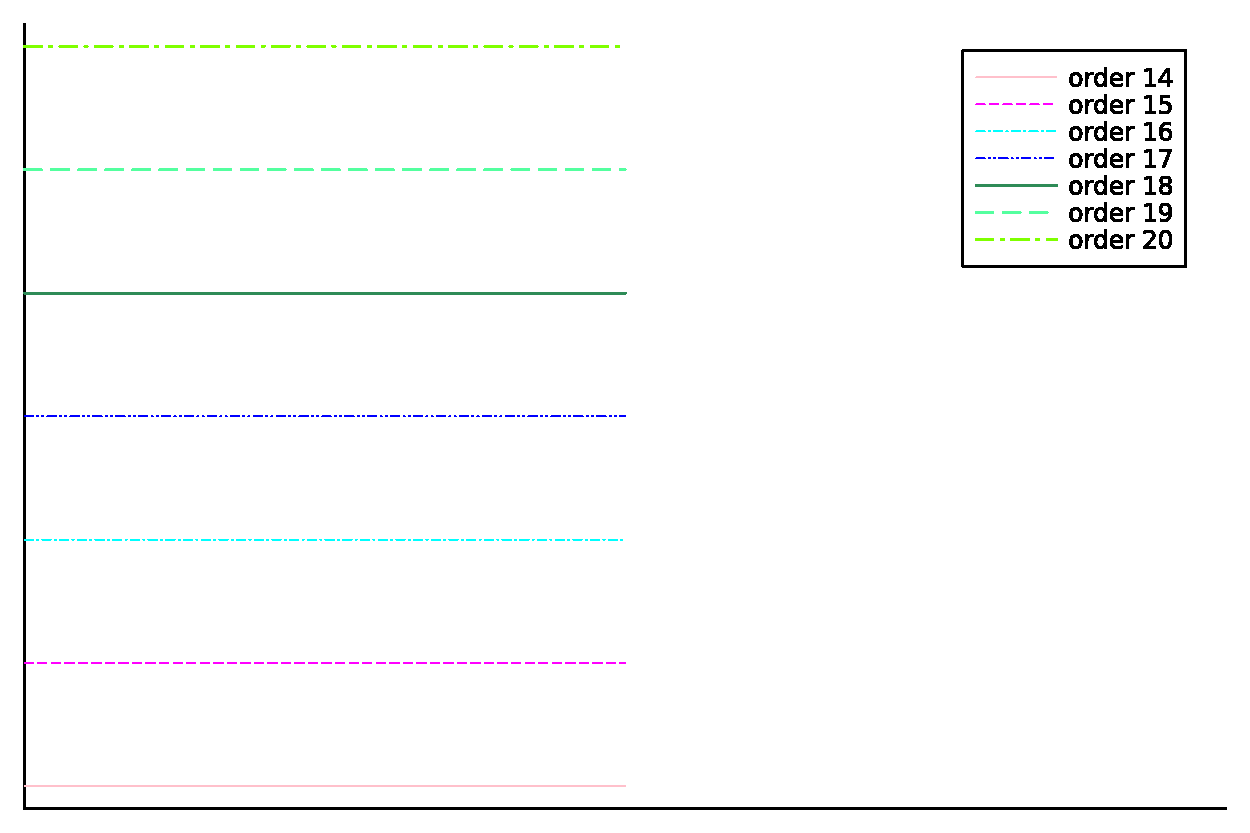
\includegraphics[width=\textwidth, trim={461 270 30 23}, clip]{pdf/odepics/colors_a-d_new_14-20.pdf}
%	\end{minipage}
%	\caption{Legend for the higher order Im sDeC methods.}
%	\label{fig: legend_high_order}
%\end{figure}

\begin{table}
	\centering
	\caption{Table with orders of the ImsDeC methods that have a bounded stability region on the negative half-plane}
	\label{tab:imsDeC_bounded}
	\begin{tabular}[h]{|c|c|}
		\hline
		ImsDeC nodes specification & orders of the method\\
		\hline
		Gauss-Lobatto & $9, 10, 11, 12, 13, 14, 15 $\\
		\hline	equispaced & $12, 13, 16, 17, 18, 19, 20 $\\
		\hline
	\end{tabular}
\end{table}
%Remark that the outlines of these stability regions can display inner or outer bounds as described before. Thereby, the shapes of these bounded stability regions mostly seem to be elliptic shaped. 
A detailed list of the bounded methods until order 20 is given in Table~\ref{tab:imsDeC_bounded}. 
%Why we use the term unbounded instead of A-stable will be discussed shortly afterwards.\\
For the sDeC, we can conclude that the choice of an implicit version does not guarantee an unbounded stability region. Nevertheless, even these implicit sDeC methods have larger stability regions than their explicit counterparts and therefore may be applicable to stiff problems. 
We notice again that this odd loss of stability in the left half plane could not be found in the ImDeC and ImADER methods. We checked it numerically up to order 50.




\begin{figure}
	\centering 
	\begin{minipage}[t]{0.45\textwidth}
		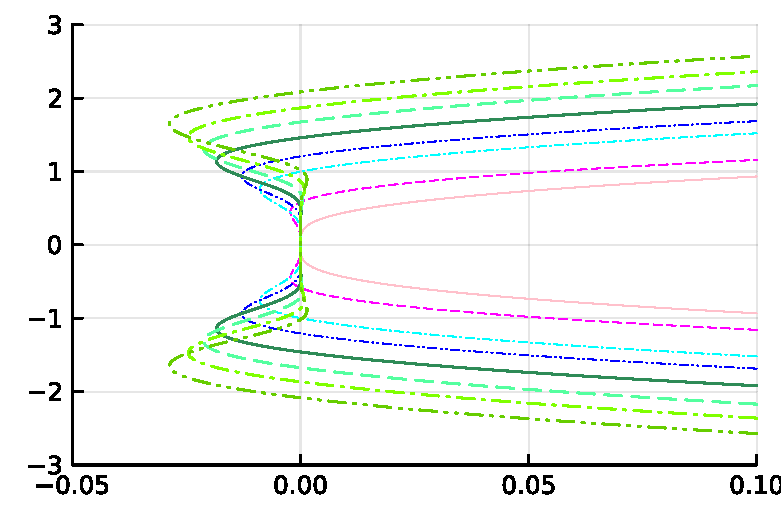
\includegraphics[width=\textwidth]{pdf/odepics/IMEXDeC_gaussLobatto_zoom.pdf}
		\centering
		ImDeC GLB from order 2 to 9
	\end{minipage}
	\begin{minipage}[t]{0.45\textwidth}
		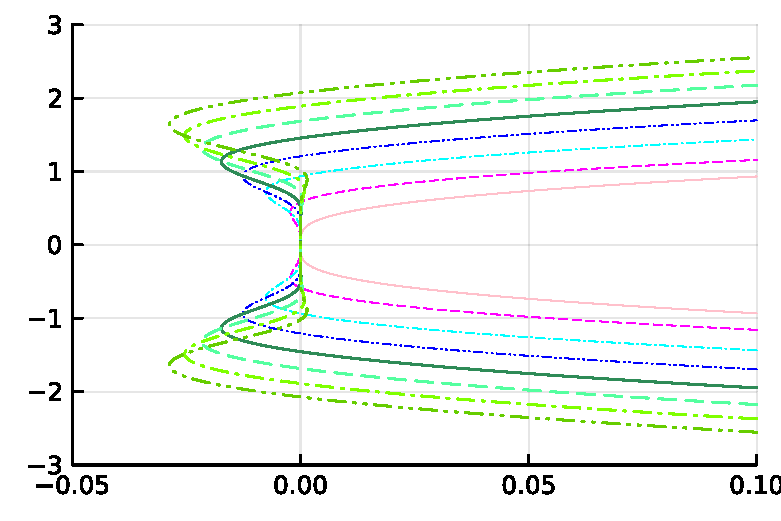
\includegraphics[width=\textwidth]{pdf/odepics/IMEXDeC_equispaced_zoom.pdf}
		\centering
		ImDeC eq from order 2 to 9
	\end{minipage}
	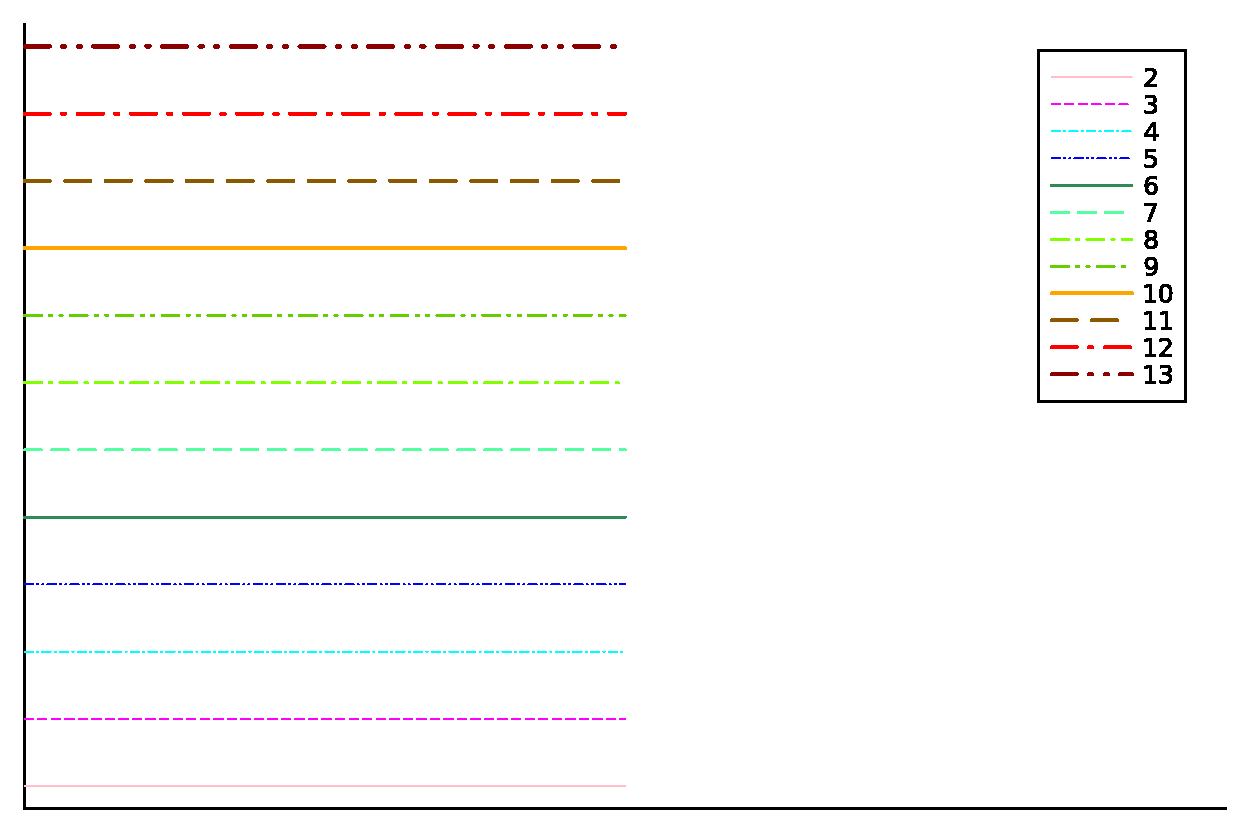
\includegraphics[width=0.08\textwidth, trim={491 140 30 23}, clip]{pdf/odepics/colors_a-d_new_2-13_no_order.pdf}\\	
	\begin{minipage}[t]{0.45\textwidth}
		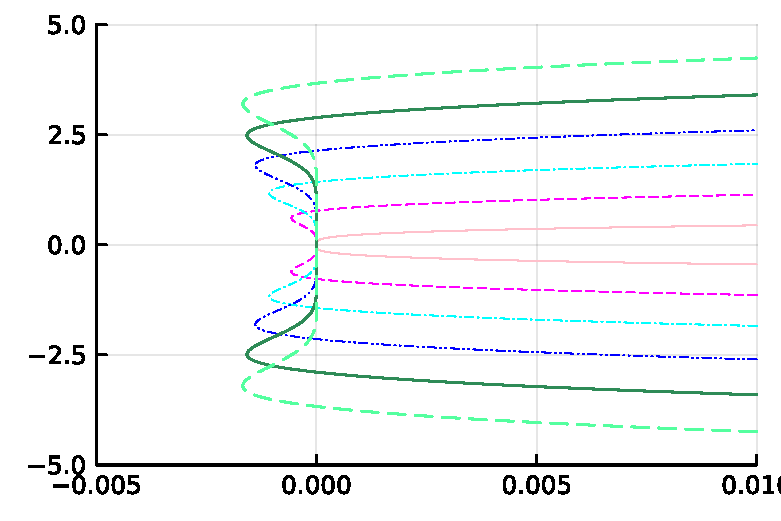
\includegraphics[width=\textwidth]{pdf/odepics/IMEXDeC_subtimesteps_gaussLobatto_zoom.pdf}
		\centering
		ImsDeC GLB from orders 2 to 7
	\end{minipage}
	\begin{minipage}[t]{0.45\textwidth}
		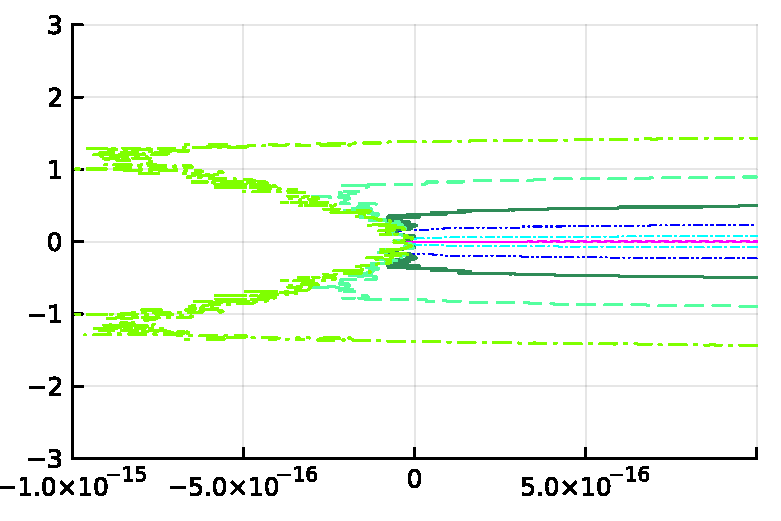
\includegraphics[width=\textwidth]{pdf/odepics/IMEXADER_equispaced_zoom.pdf}
		\centering
		ImADER eq from orders 3 to 8
	\end{minipage}
	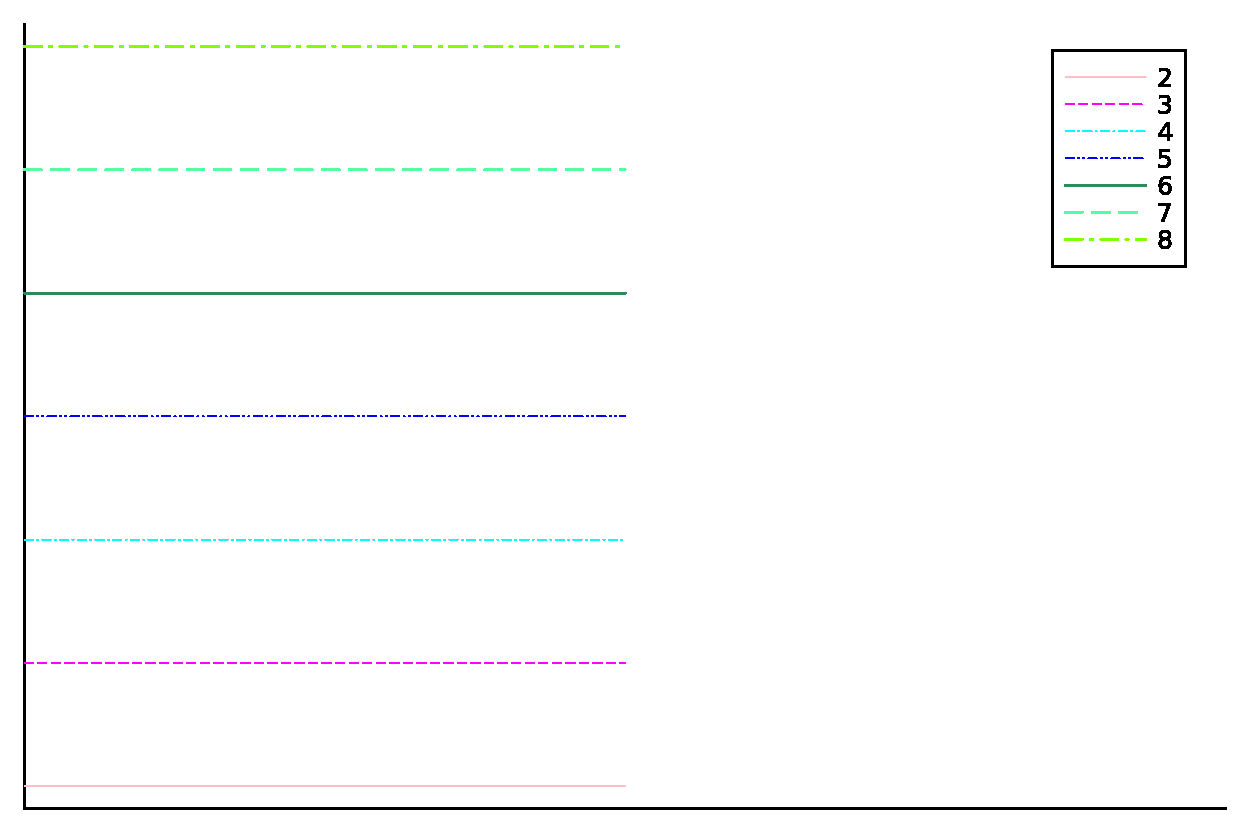
\includegraphics[width=0.08\textwidth, trim={491 180 30 23}, clip]{pdf/odepics/colors_a-d_new_2-8_no_order.pdf}
	\caption{Zoomed stability region of various implicit schemes}
	\label{fig: ODE_minor_instabilitys}
\end{figure}

Taking a closer look at the implicit methods, we additionally detect some minor instability regions on the negative half-plane, see Figure~\ref{fig: ODE_minor_instabilitys}.
It turns out that these instabilities appear for all ImDeC and ImsDeC methods of orders larger than 2 and both types of nodes. We display the sDeC only with GLB nodes, as the equispaced nodes version is very similar to that.
For a very small scale, the same can be seen for the ImADER methods with equispaced nodes of orders at least larger than 4, displayed on the bottom right of Figure~\ref{fig: ODE_minor_instabilitys}. 
Notice that the sizes of the unstable regions are close to machine precision, which results in non-smooth boundaries and it is unclear if the ImADER with equispaced nodes of order 3 and 4 
are A-stable or not. \todo{Suggestion delete equidsitand nodes and bring everyhing in figure 3 in one line.. }

As proved in Section~\ref{subsec:ADER_A-stability}, also numerically we observe that the ImADER methods with Gauss-Lobatto nodes are A-stable for all orders. 

%Hence, we classify the implicit methods as A-stable, \textit{almost A-stable}, when the stability region is unbounded and it \textit{almost} includes the whole left half--plane, or with bounded stability region.
%Remark that for \textit{almost A-stable} methods these minor instabilities do not influence the behavior of the scheme on many stiff problems. Nevertheless, when the eigenvalues $\lambda$ of the system are (almost) purely imaginary, they might encounter instabilities for some discretizations.
%, so that for certain step-sizes $\Delta t$ it is possible to get a $z=\lambda \Delta t$ located in the unstable region.


Summarizing, we can categorize our methods in 3 different classes: The A-stable schemes, \textit{almost A-stable} schemes, when the stability region is unbounded and it \textit{almost} includes the whole left half--plane, and the non-A-stable schemes. 
While only the implicit ADER methods with Gauss-Lobatto nodes are A-stable, we saw that the ADER methods with equispaced nodes and all DeC methods are almost A-stable by just possessing some minor instabilities on the negative half-plane around the origin. 
For the sDeC methods, we even have bounded stability regions for some higher orders which make them clearly non-A-stable, while the remaining sDeC schemes also belong into the category of almost-A-stable methods. \todo{maybe a itemize or something minipages...}

Remark that for \textit{almost A-stable} methods these minor instabilities do not influence the behavior of the scheme on many stiff problems. Nevertheless, when the eigenvalues $\lambda$ of the system are (almost) purely imaginary, they might encounter instabilities for some discretizations.

\subsection{IMEX schemes}
To study the stability of IMEX schemes, we will use the RK stability function 
%We will now evaluate our constructed IMEX methods, by using their Butcher tableaux 
%\begin{equation}\label{eq:ImExButcherTableu}
%\begin{array}{c|c}
%c & A\\\hline
%& b^T
%\end{array}, \qquad
%\begin{array}{c|c}
%c & \hat{A}\\\hline
%& \hat{b^T}
%\end{array}.
%\end{equation}
%to receive their stability functions
\begin{equation}\label{eq:ImExStabilityFunction}
R(z_I, z_E)=1+\left(z_I\vec{b}^T+z_E\vec{\hat{b}}^T\right)\vec{u}=1+\left(z_I\vec{b}^T+z_E\vec{\hat{b}}^T\right)\left(\mat{Id}-z_I\mat{A}-z_E\mat{\hat{A}}\right)^{-1} \vec{1}
\end{equation}
that uses the matrices defined by the Butcher tableau of an IMEX RK \eqref{eq:IMEX_Butcher}.
Remark that the standard approach of A-stability cannot be used anymore.
Indeed, the region of absolute stability $$S=\left\{(z_I,z_E)\in \mathbb{C}^2 \ : \ \lvert{R(z_I,z_E)}\rvert\le1\right\}$$ lays in a larger space, with respect to classical RK schemes, therefore, its study, computation and visualization are challenging.
%Like in the classic case, we do not need (and do not want) the whole region $\mathbb{C}^2$ for satisfying results besides the issue of problematic visualization. Here arises the question which subsets of stability we want to consider. \\
Hence, we need to rely on some simplifications.
In \cite{minion2003dec}, Minion simplifies the Dahlquist equation by imposing
\begin{equation*}
\lambda_I \in \mathbb{R}, \quad \lambda_E =i\lambda_E', \ \lambda_E' \in \mathbb{R}.
\end{equation*} 
This procedure neglects respectively the imaginary or real part of the coefficients in the Dahlquist equation to display a two-dimensional region. This idea is lead by classical PDE discrete operators, where typically the diffusion is symmetric negative definite, while the advection is mainly with imaginary eigenvalues. 
A second approach where for each $\lambda_E$ the A-stability is required for the implicit part of the scheme was originally studied in \cite{zhong1996additive,caflisch1997uniformly} and formalized in \cite{liotta2000central}. Another approach studies, instead, the stability for each $\lambda_I$ requiring at least the stability region of the explicit Euler method to the explicit part \cite{Hundsdorfer}.
We collect these definitions of stability region in the following.
\begin{definition}[Stability regions]
	Consider the modified test equation with stability function \eqref{eq:ImExStabilityFunction}. Then, we define multiple approaches for IMEX stability regions by
	\begin{itemize}
		\item $S:=\left\{(z_I,z_E)\in \mathbb{C}^2 \ :\ \lvert{R(z_I,z_E)}\rvert\le1\right\}$ (Region of absolute stability),
	\item  $\mathcal{D}_M:= \left\{(z_I,z_E)\in \mathbb{R}^2 \ :\ \lvert{R(z_I,iz_E)}\rvert\le1\right\}$  (Minion's stability region) \cite{minion2003dec}, 
	\item  $\mathcal{D}_0:=\left\{z_E \in \mathbb{C}\ :\ \lvert{R(z_I,z_E)}\rvert \le 1 \textrm{ for any } z_I \in \mathbb{C}^- \right\}$ \cite{liotta2000central},
	\item $\mathcal{D}_1:=\left\{z_I \in \mathbb{C}\ :\ \lvert{R(z_I,z_E)}\rvert \le 1 \textrm{ for any } z_E \in \mathcal{S}_0 \right\}$ \cite{Hundsdorfer},
	\end{itemize}
	where $\mathcal{S}_0=\left\{z_E \in \mathbb{C}\ :\ \lvert 1+z_E\rvert \le 1 \right\}$ is the stability region of the explicit Euler method. 
\end{definition}
%Remark that $\mathbb{C}^-$ is the smallest stability region to fulfill the A-stability. 
%Hundsdorfer's definitions \cite{Hundsdorfer} $\mathcal{D}_0$ and $\mathcal{D}_1$ give statements about the explicit or implicit part of the equation, respectively assuming that the other part fulfills these known stability properties.
$\mathcal D_0$ is a very strict condition of IMEX stability, in particular for the considered high order schemes. 
%We will refer to $\mathcal{D}_M$ as Minion's stability approach and to $\mathcal{D}_0$ /\mathcal{D}_1$ as Hundsdorfer's stability approach.
Theoretically, the terms A-stability and A($\alpha$)-stability may be applied for all 3 of these subsets of $\mathbb{C}$ analogously to the classical cases, so we will make use of this terminology too. 

\subsubsection*{$\mathcal{D}_M$ stability region}
\begin{figure}
	\centering
	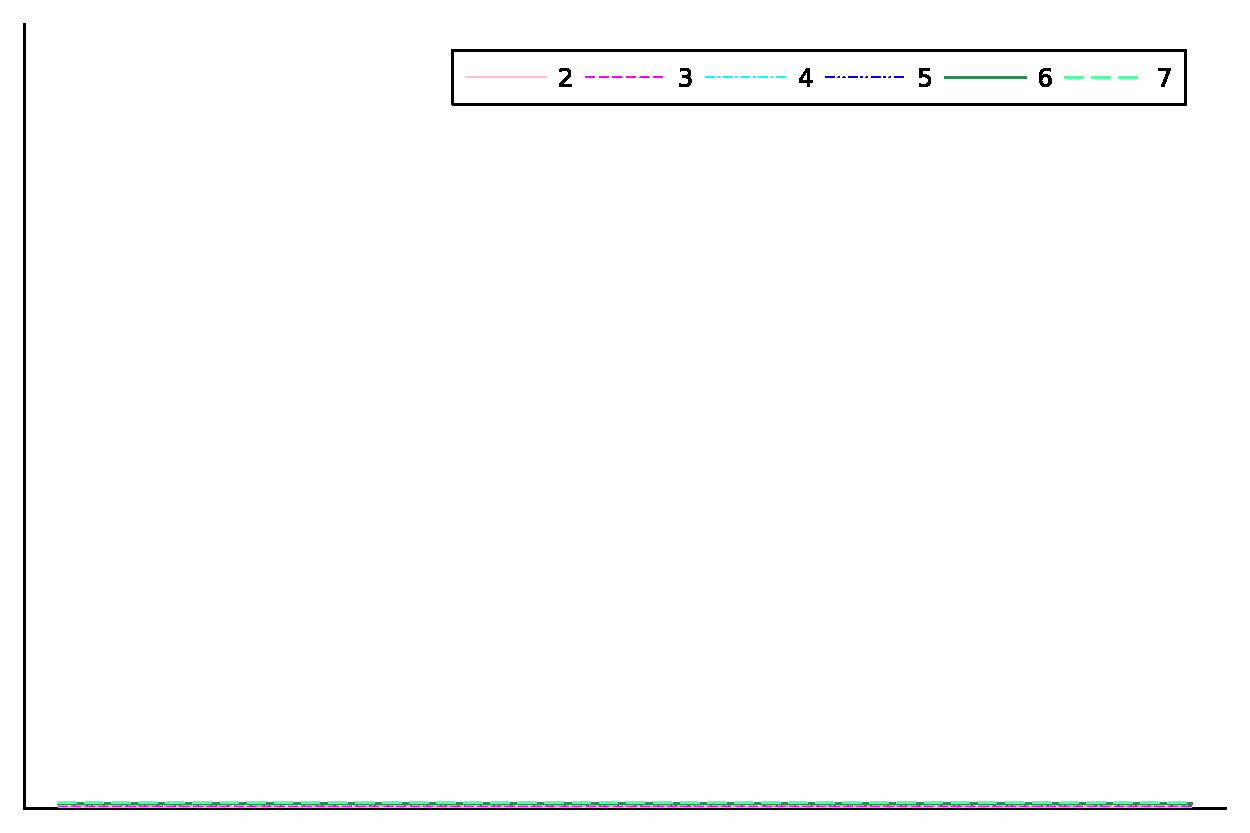
\includegraphics[width=0.465\textwidth,trim={215 340 32 22}, clip]{pdf/odepics/colors_a-d_new_horiz_2-7_no_order.pdf}\!\!
	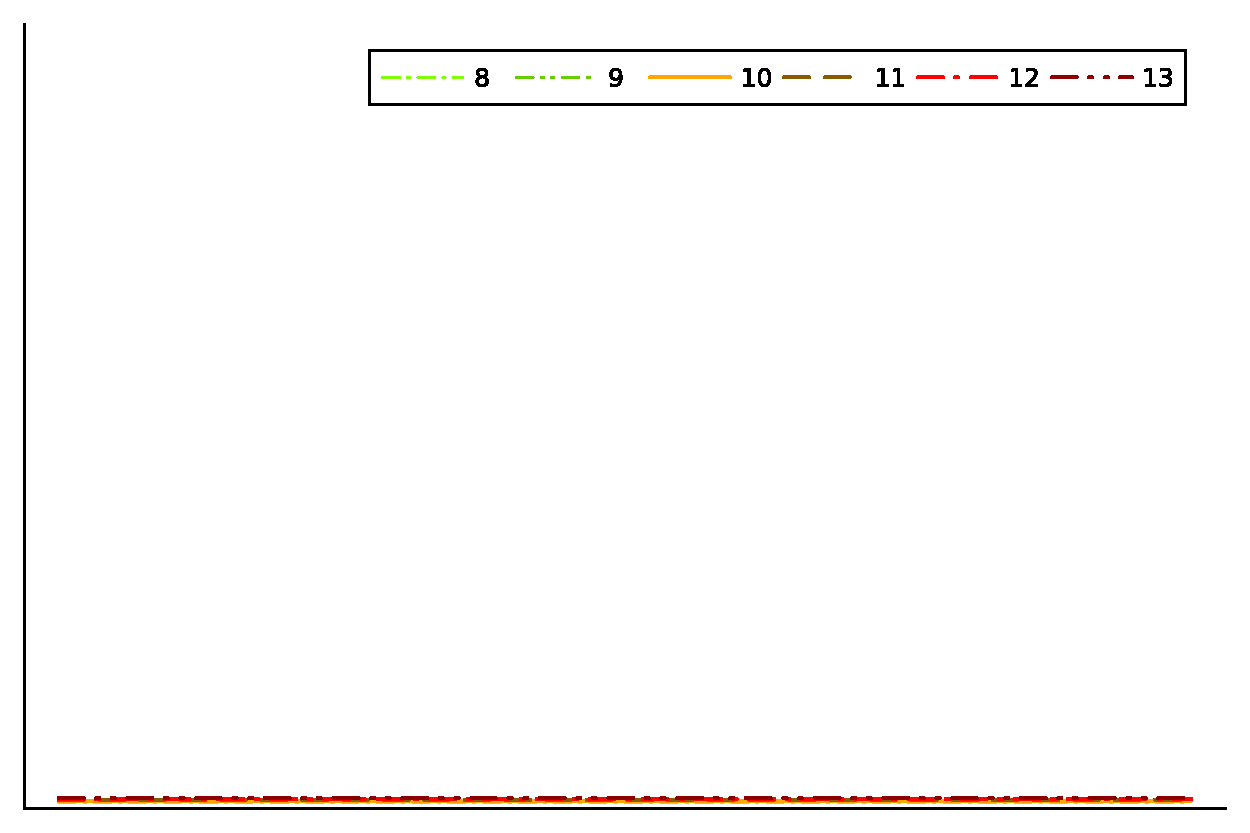
\includegraphics[width=0.515\textwidth,trim={178 340 30 22}, clip]{pdf/odepics/colors_a-d_new_horiz_8-13_no_order.pdf}\\
	\begin{minipage}[t]{0.32\textwidth}
		\centering
		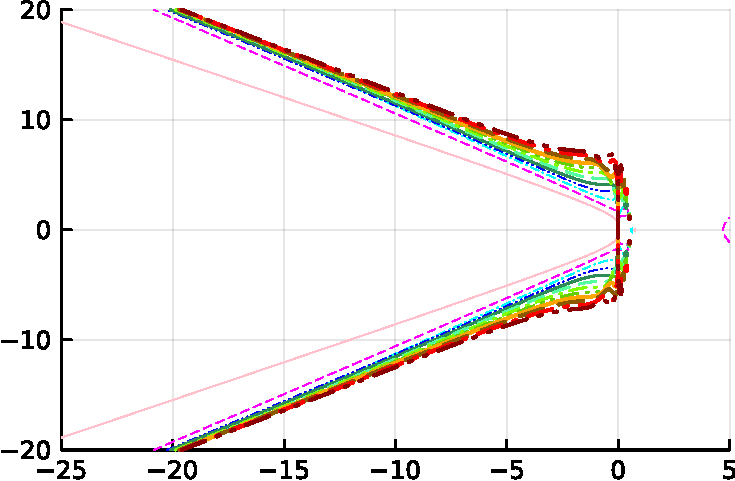
\includegraphics[width=\textwidth, trim={0 0 0 22}, clip]{pdf/odepics/Minion_IMEXDeC_eq_ord13-crop.pdf}
		IMEXDeC eq orders 2 to 13
	\end{minipage}	
	\begin{minipage}[t]{0.32\textwidth}
		\centering
		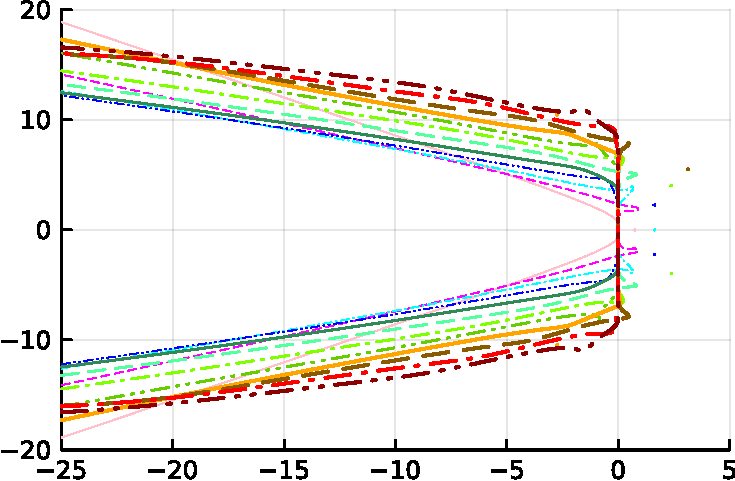
\includegraphics[width=\textwidth, trim={0 0 0 22}, clip]{pdf/odepics/Minion_IMEXsDeC_eq_ord13-crop.pdf}
		IMEXsDeC eq orders 2 to 13
	\end{minipage}
	\begin{minipage}[t]{0.32\textwidth}
		\centering
		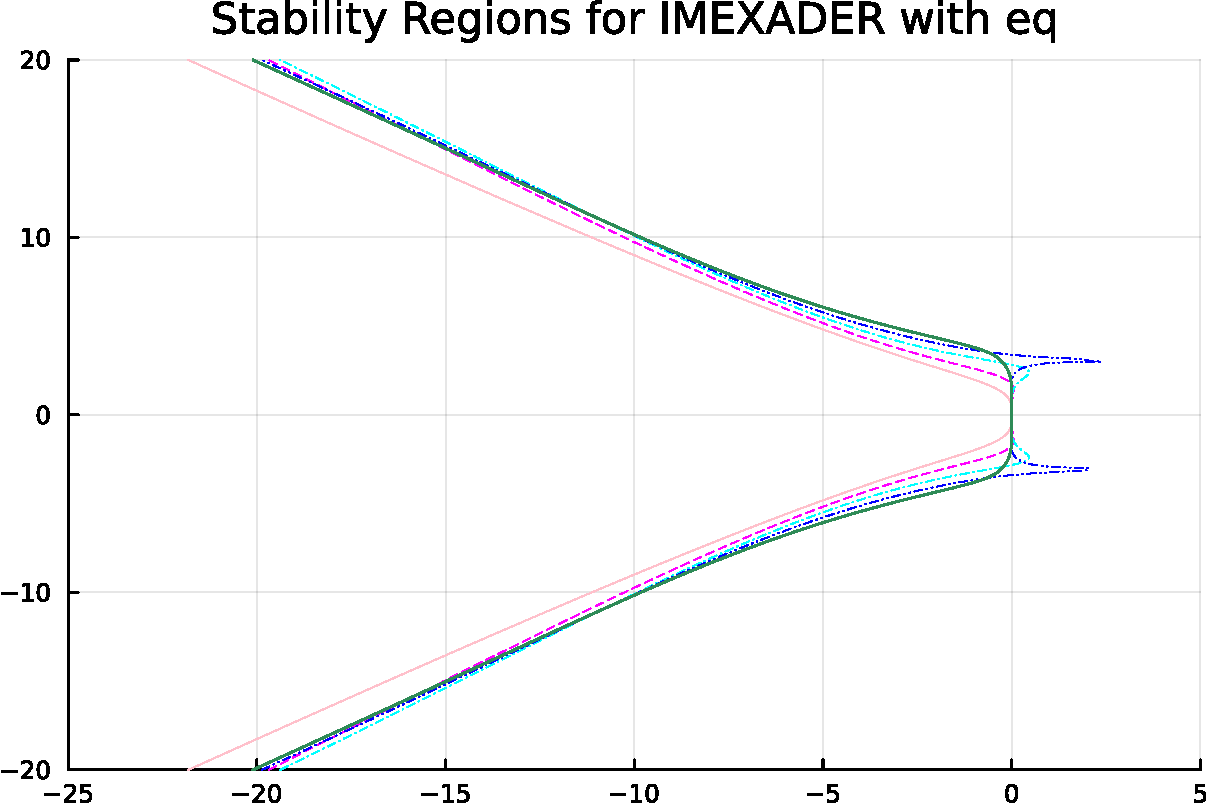
\includegraphics[width=\textwidth, trim={0 0 0 22}, clip]{pdf/odepics/Minion_IMEXADER_eq_ord6-crop.pdf}
		IMEXADER eq orders 2 to 6
	\end{minipage}\\
	\begin{minipage}[t]{0.32\textwidth}
		\centering
		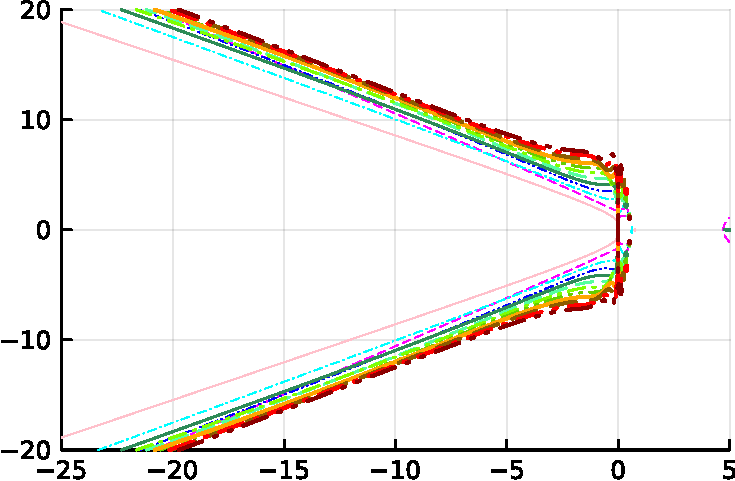
\includegraphics[width=\textwidth, trim={0 0 0 22}, clip]{pdf/odepics/Minion_IMEXDeC_GLB_ord13-crop.pdf}
		IMEXDeC GLB orders 2 to 13
	\end{minipage}
	\begin{minipage}[t]{0.32\textwidth}
		\centering
		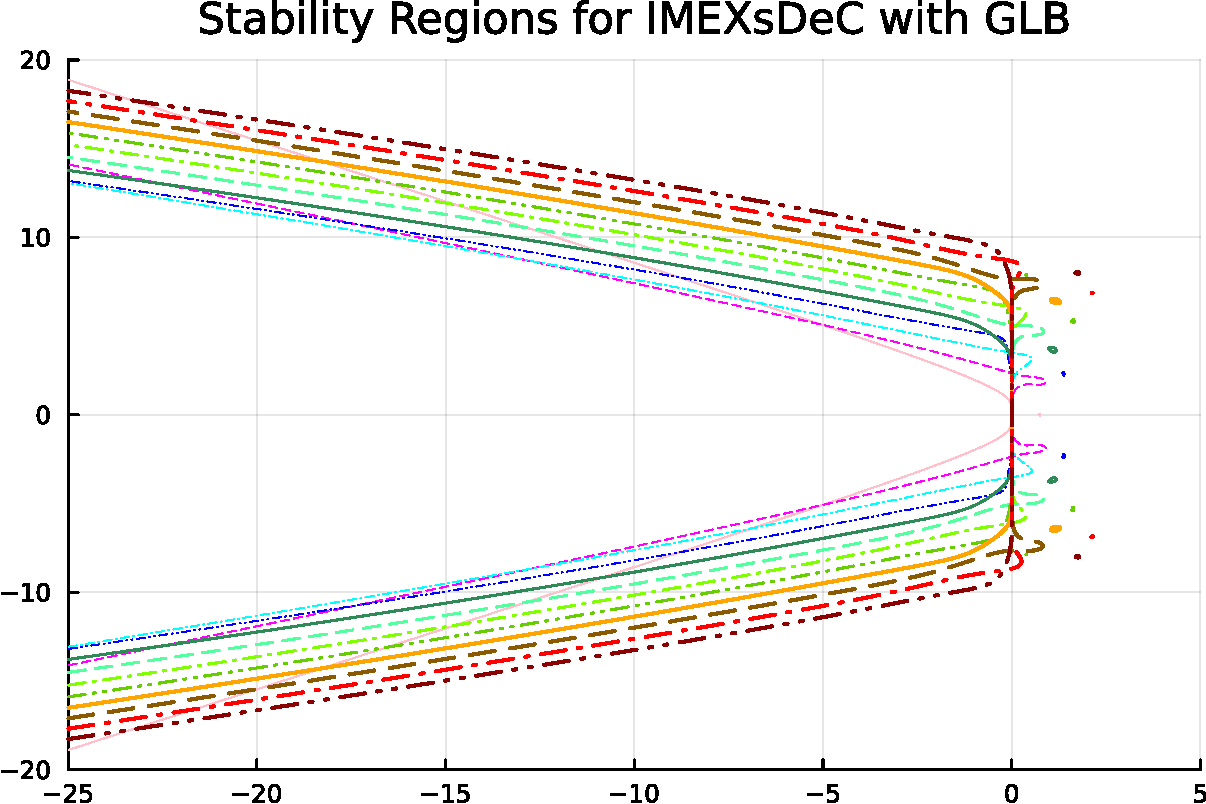
\includegraphics[width=\textwidth, trim={0 0 0 22}, clip]{pdf/odepics/Minion_IMEXsDeC_GLB_ord13-crop.pdf}
		IMEXsDeC GLB orders 2 to 13
	\end{minipage}
	\begin{minipage}[t]{0.32\textwidth}
		\centering
		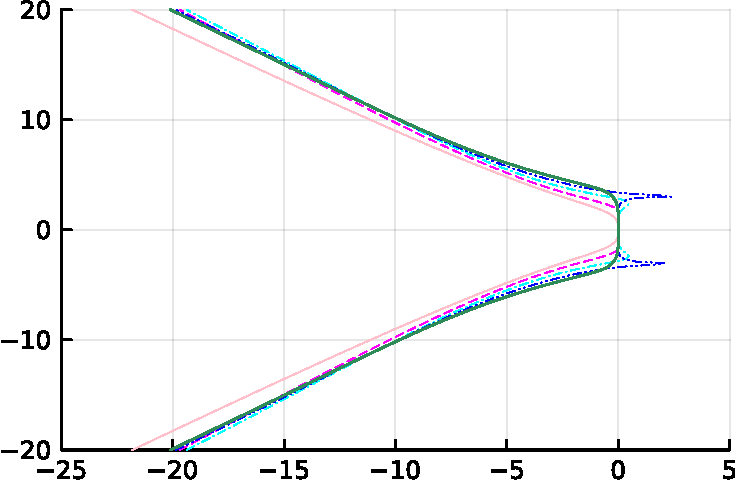
\includegraphics[width=\textwidth, trim={0 0 0 22}, clip]{pdf/odepics/Minion_IMEXADER_GLB_ord6-crop.pdf}
		IMEXADER GLB orders 2 to 6
	\end{minipage}
	\caption{Minion's stability region for IMEX DeC (left), sDeC (center) and ADER (right) with equispaced (top) and GLB (bottom) nodes}
	\label{fig: ODEIMEX}
\end{figure}
We recall that the plots of the stability regions have very different meaning according to the chosen approach. 
%Considering the previously developed IMEX methods, we want to recall that the view on the regions of stability changes, depending on the approach we choose. Firstly, we want to consider stability like in \cite{minion2003dec}. 
%It is possible to write the method used there into the IMEX sDeC method, so we expect the same results as him in \cite[fig. 4.1]{minion2003dec}. 
Starting from Minion's approach \cite{minion2003dec}, we evaluate the IMEX stability function \eqref{eq:ImExStabilityFunction} numerically to calculate the respective stability regions. 

For the IMEX DeC, we can observe in Figure~\ref{fig: ODEIMEX} (left) that the choice of nodes change the regions on some details but the qualitative behavior is the same. We can also conclude on an $A(\alpha)-$stability for approximately $\alpha=35^\circ$.

Going on to the IMEX ADER, we can see in Figure~\ref{fig: ODEIMEX} (right) a similar behavior, even if the stability regions differ in small details, we observe $A(\alpha)-$stability for at least $\alpha=35^\circ$.

Finally, for the IMEX sDeC method in Figure~\ref{fig: ODEIMEX} (center) we see a slightly different behavior, still resulting in an $A(\alpha)-$stability, but for significantly smaller angles, approximately $\alpha=18^\circ$. 
%Remark that this is significantly lower than for both the IMEX ADER and IMEX DeC. 
Nevertheless, the result on the bottom center in Figure~\ref{fig: ODEIMEX} with GLB nodes coincides with the one in \cite{minion2003dec}, as expected. 
%So we can conclude that the IMEX variations for all of these methods also have a somehow similar $A(\alpha)-$stability for some $\alpha>10^\circ$, at least for this view on the stability for IMEX methods.\\
It is also noticeable that the IMEX sDeC stability region of order 2 is $A(\alpha)$-stable with larger $\alpha$ as it coincides with the IMEX DeC2.


\subsubsection*{$\mathcal{D}_0$ stability region}

Now, we want to evaluate $\mathcal{D}_0$ stability for our IMEX methods. 
We want to emphasize that the requirements here are stricter than in Minion's approach. 
Indeed, for $\mathcal{D}_0$ we require the method to be at least fully A-stable for the implicit part and we look at the stability of the explicit part.

The IMEX DeC and IMEX sDeC have $\mathcal{D}_0=\emptyset$ and this is probably related to the fact that their implicit counterpart is not A-stable.
For the IMEX ADER, only few orders have non-empty $\mathcal{D}_0$ stability region. In Figure~\ref{fig: HundsdorferD0_IMEXADER}, we show the few stability regions, which eventually vanish when increasing the order of accuracy.
\begin{figure}
	\centering
	\begin{minipage}[t]{0.45\textwidth}
		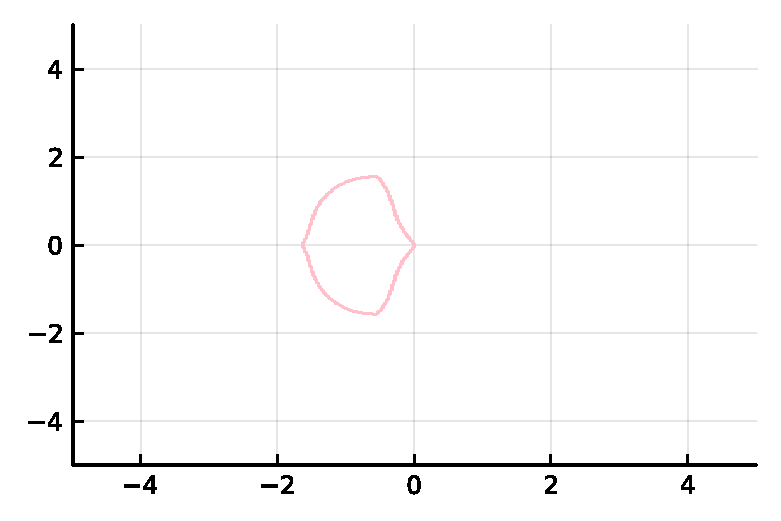
\includegraphics[width=\textwidth]{pdf/odepics/ImExD0_IMEXADER_equispaced.pdf}
		\centerline{Order 2 with equispaced nodes}
	\end{minipage}
	\begin{minipage}[t]{0.45\textwidth}
		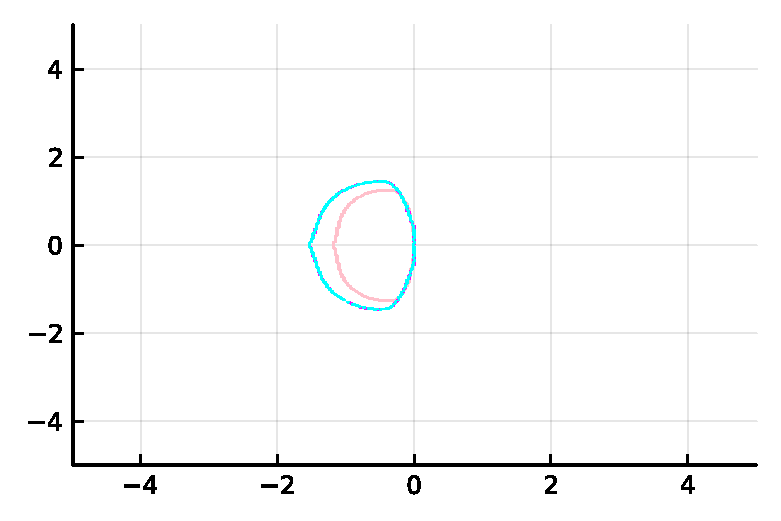
\includegraphics[width=\textwidth]{pdf/odepics/ImExD0_IMEXADER_gaussLobatto.pdf}
		\centerline{Orders 2 to 4 with Gauss-Lobatto nodes}
	\end{minipage}
	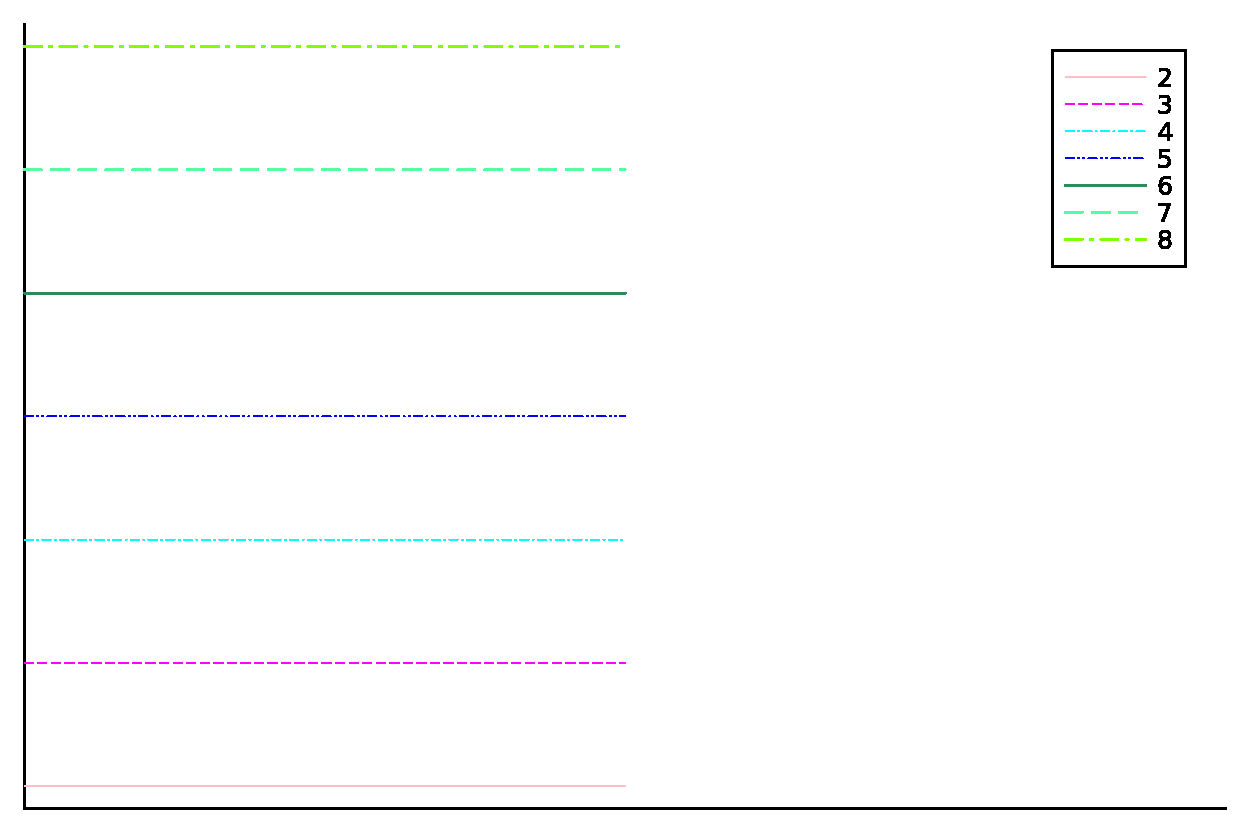
\includegraphics[width=0.08\textwidth, trim={491 180 30 23}, clip]{pdf/odepics/colors_a-d_new_2-8_no_order.pdf}
	\caption{$\mathcal{D}_0$ Stability regions for IMEX ADER. The smaller stability region displays order 2, while the larger one displays order 3 and 4 (right)}
\label{fig: HundsdorferD0_IMEXADER}
\end{figure}

\subsubsection*{$\mathcal{D}_1$ stability region}
We plot the $\mathcal{D}_1$ stability regions for DeC and sDeC methods in Figures~\ref{fig: HundsdorferD1_IMEX}, where we require the explicit part to cover the stability region of the explicit Euler method and we look at the stability of the implicit part. 
Contrary to the $\mathcal{D}_0$ cases, we observe non-empty, limited regions of stability for every order for the IMEX DeC methods. Moreover, there is no regularity in their shape and their size grow significantly as the order of accuracy increases.
Notice that the plots do not show the full stability regions of higher orders, for example for orders 6, 7, and 8 with equispaced nodes, but they are anyway bounded regions. \\
For the IMEX sDeC, see Figure~\ref{fig: HundsdorferD1_IMEX} (center), we observe some remarkable differences. In the case of equispaced nodes, even orders just show the small bounded stability regions in the negative half-plane nearby the origin, odd orders smaller than 6 show large stability regions, while they are unstable starting from order 7. 
Also in the GLB case, we do not observe much regularity. 
We notice that the largest stability region is obtained for order 5, while, for higher orders, the stability region almost fit in the plot.
\begin{figure}
	\centering
	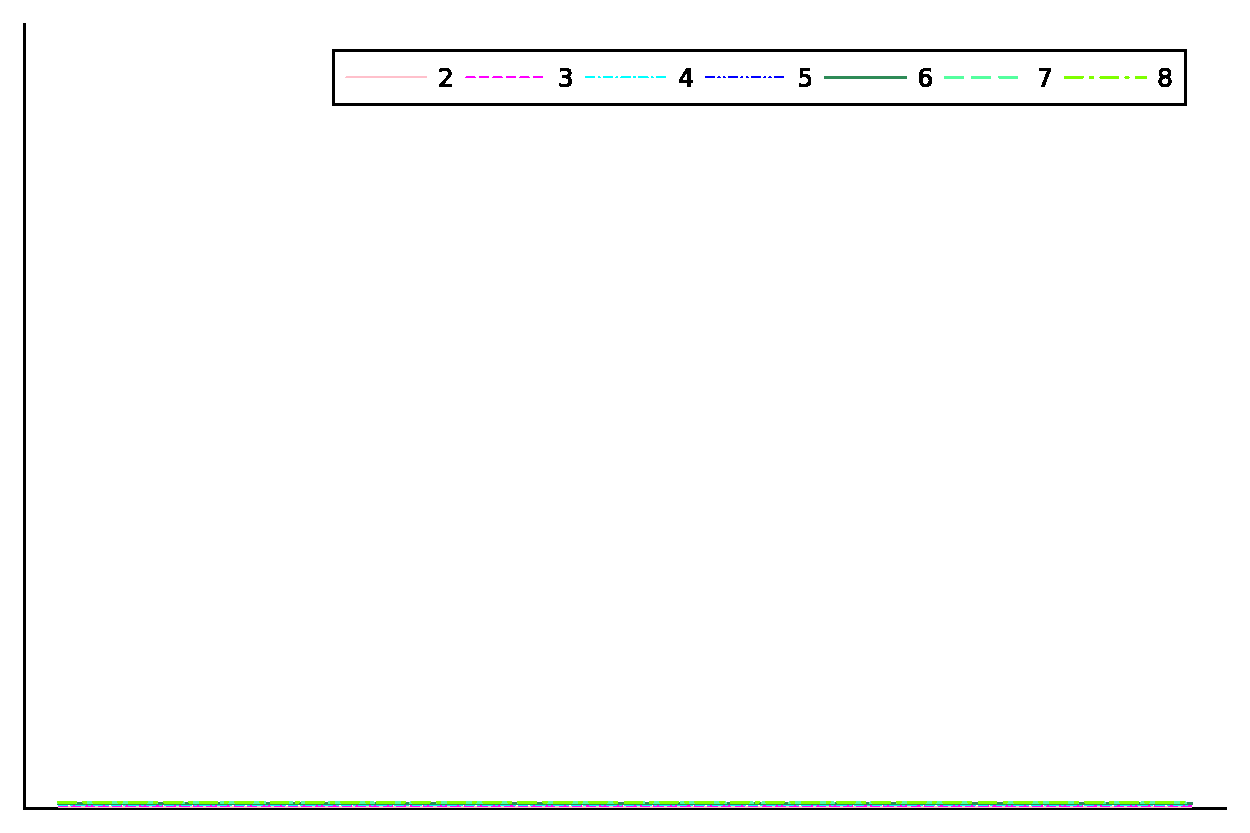
\includegraphics[width=0.515\textwidth,trim={158 340 30 22}, clip]{pdf/odepics/colors_a-d_new_horiz_2-8_no_order.pdf}\\
	\begin{minipage}[t]{0.32\textwidth}
		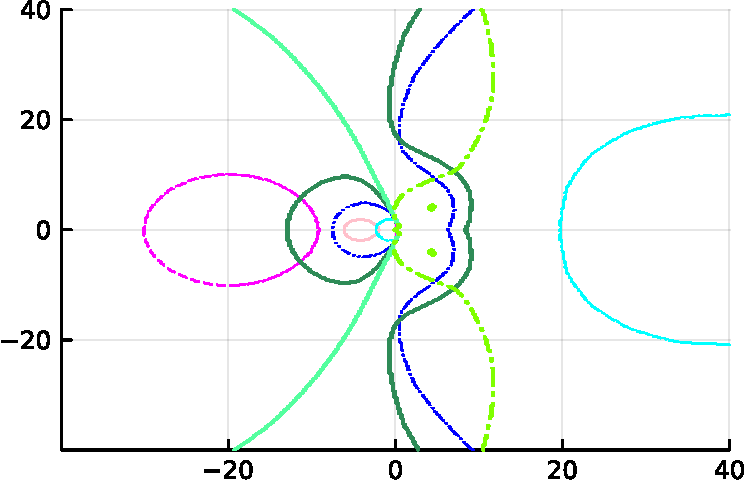
\includegraphics[width=\textwidth]{pdf/odepics/ImExD1_IMEXDeC_equispaced_range=40-crop.pdf}
		\centerline{IMEX DeC eq}
	\end{minipage}
	\begin{minipage}[t]{0.32\textwidth}
	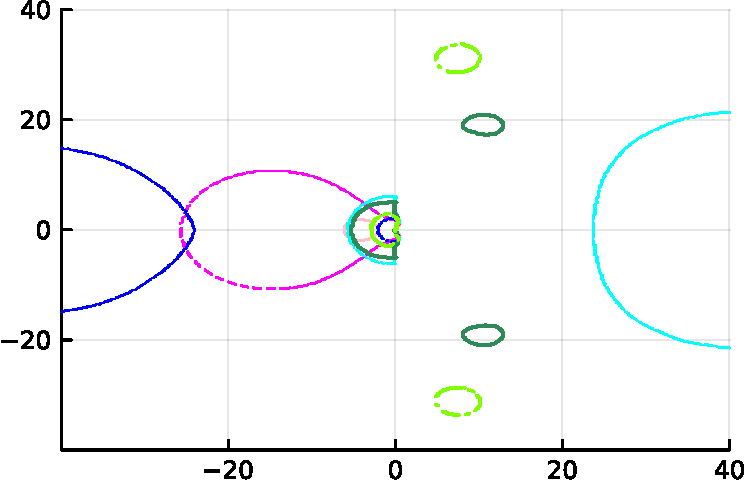
\includegraphics[width=\textwidth]{pdf/odepics/ImExD1_IMEXDeC_subtimesteps_equispaced_range=40-crop.pdf}
	\centerline{IMEX sDeC eq}
	\end{minipage}
	\begin{minipage}[t]{0.32\textwidth}
	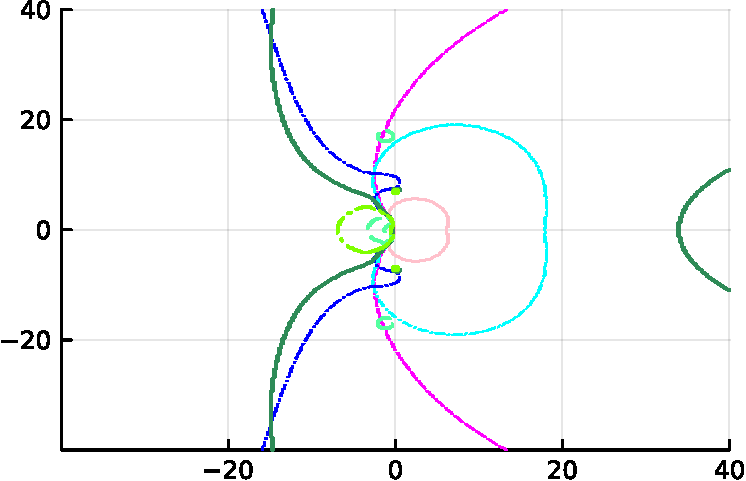
\includegraphics[width=\textwidth]{pdf/odepics/ImExD1_IMEXADER_equispaced_range=40-crop.pdf}
	\centerline{IMEX ADER eq}
	\end{minipage}\\
	\begin{minipage}[t]{0.32\textwidth}
	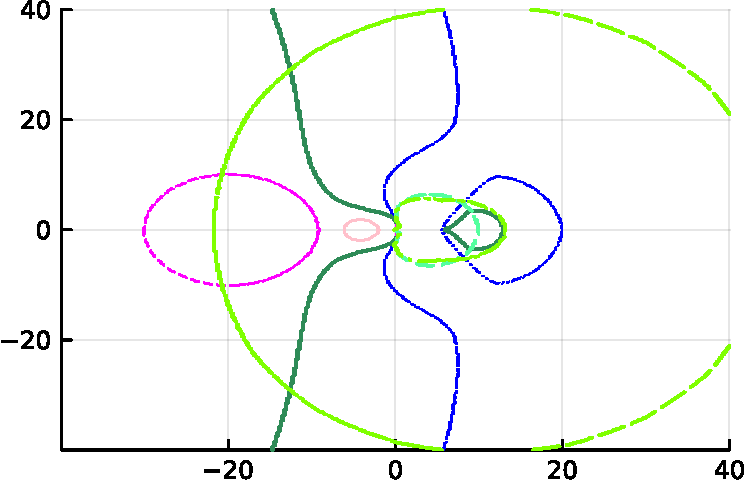
\includegraphics[width=\textwidth]{pdf/odepics/ImExD1_IMEXDeC_gaussLobatto_range=40-crop.pdf}
	\centerline{IMEX DeC GLB}
	\end{minipage}
	\begin{minipage}[t]{0.32\textwidth}
	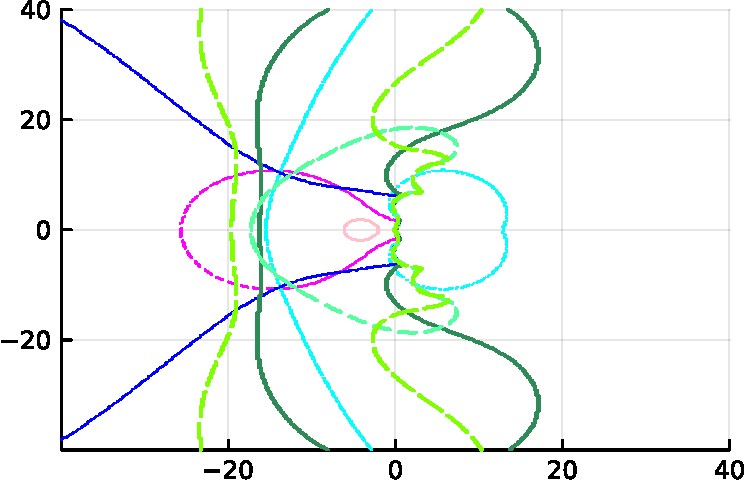
\includegraphics[width=\textwidth]{pdf/odepics/ImExD1_IMEXDeC_subtimesteps_gaussLobatto_range=40-crop.pdf}
	\centerline{IMEX sDeC GLB}
	\end{minipage}
	\begin{minipage}[t]{0.32\textwidth}
	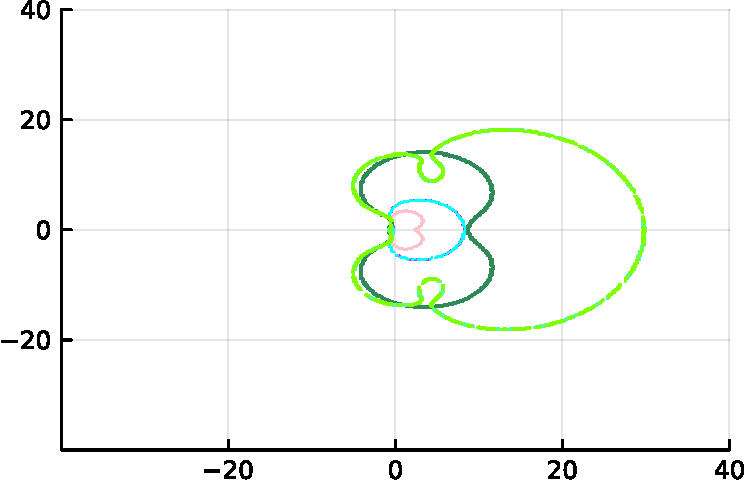
\includegraphics[width=\textwidth]{pdf/odepics/ImExD1_IMEXADER_gaussLobatto_range=40-crop.pdf}
	\centerline{IMEX ADER GLB}
	\end{minipage}
%	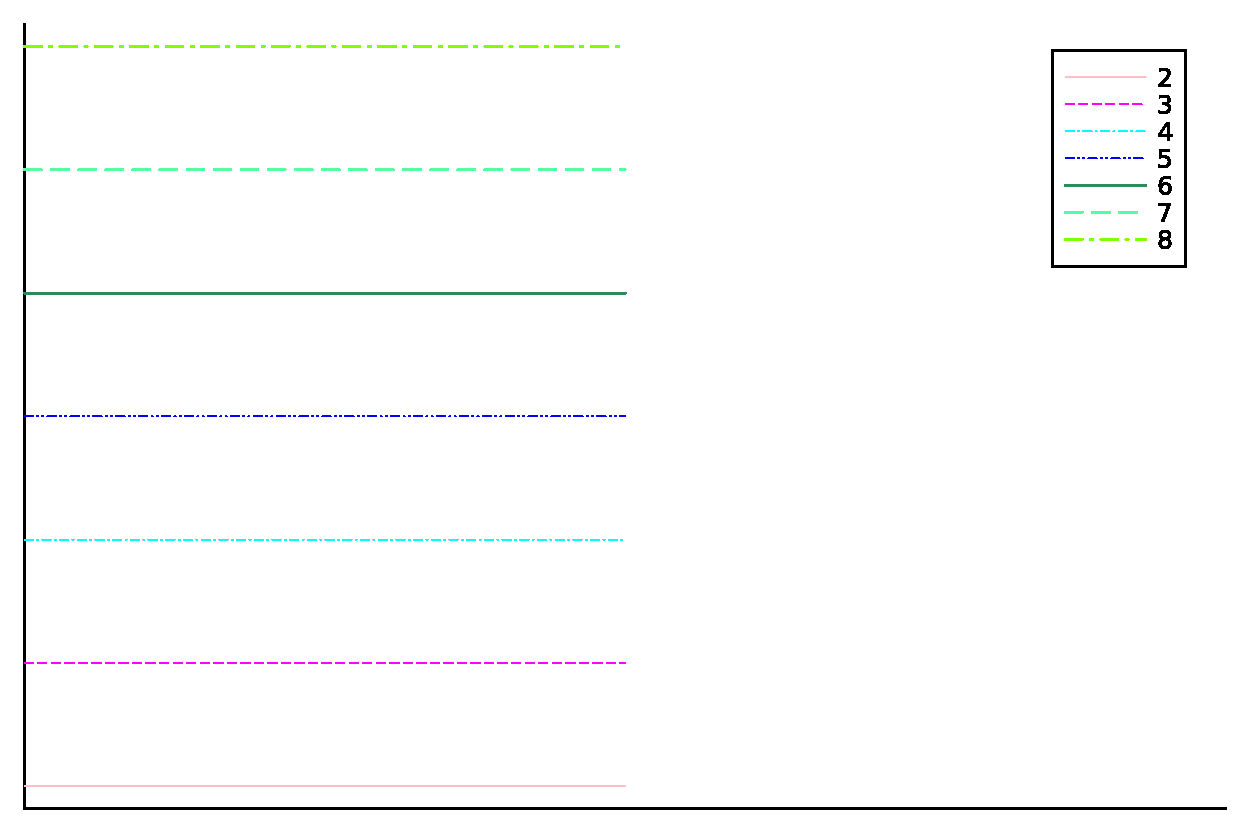
\includegraphics[width=0.08\textwidth, trim={491 180 30 23}, clip]{pdf/odepics/colors_a-d_new_2-8_no_order.pdf}
	\caption{$\mathcal{D}_1$ Stability Region for IMEX DeC (left), sDeC (center) and ADER (right) with equispaced (top) and GLB (bottom) nodes: orders 2 to 8}
\label{fig: HundsdorferD1_IMEX}
\end{figure}

%\begin{figure}
%	\centering
%	\begin{minipage}[t]{0.45\textwidth}
%		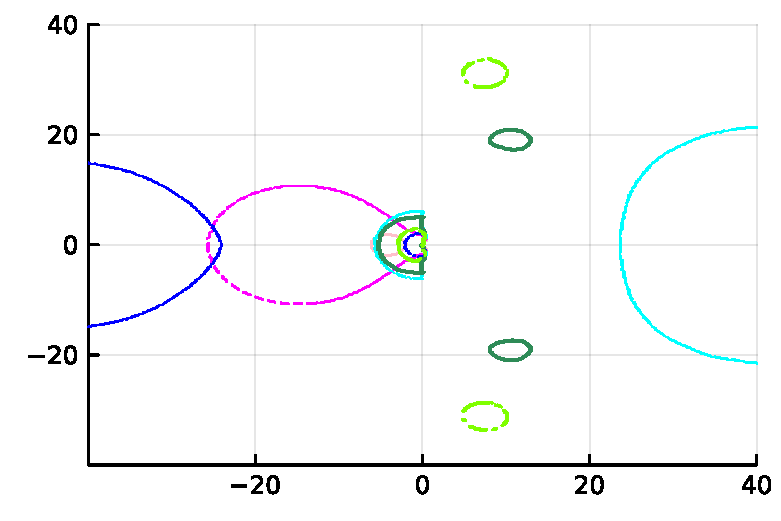
\includegraphics[width=\textwidth]{pdf/odepics/ImExD1_IMEXDeC_subtimesteps_equispaced_range=40.pdf}
%		\centerline{equispaced nodes}
%	\end{minipage}
%	\begin{minipage}[t]{0.45\textwidth}
%		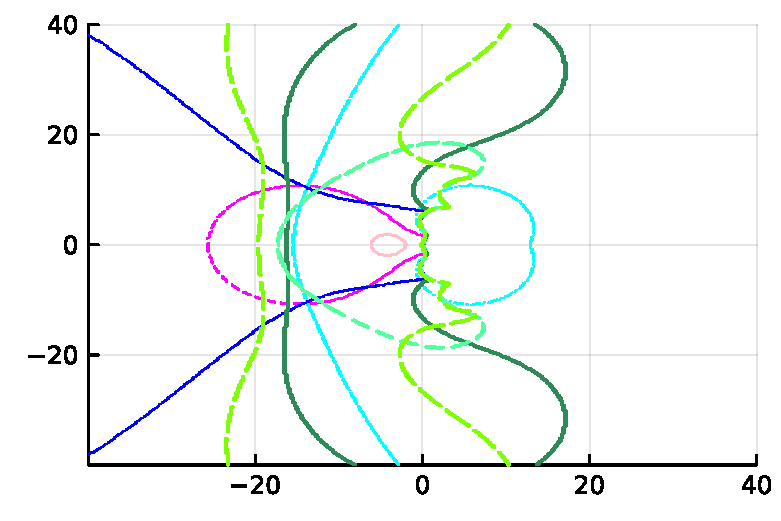
\includegraphics[width=\textwidth]{pdf/odepics/ImExD1_IMEXDeC_subtimesteps_gaussLobatto_range=40.pdf}
%		\centerline{Gauss-Lobatto nodes}
%	\end{minipage}
%	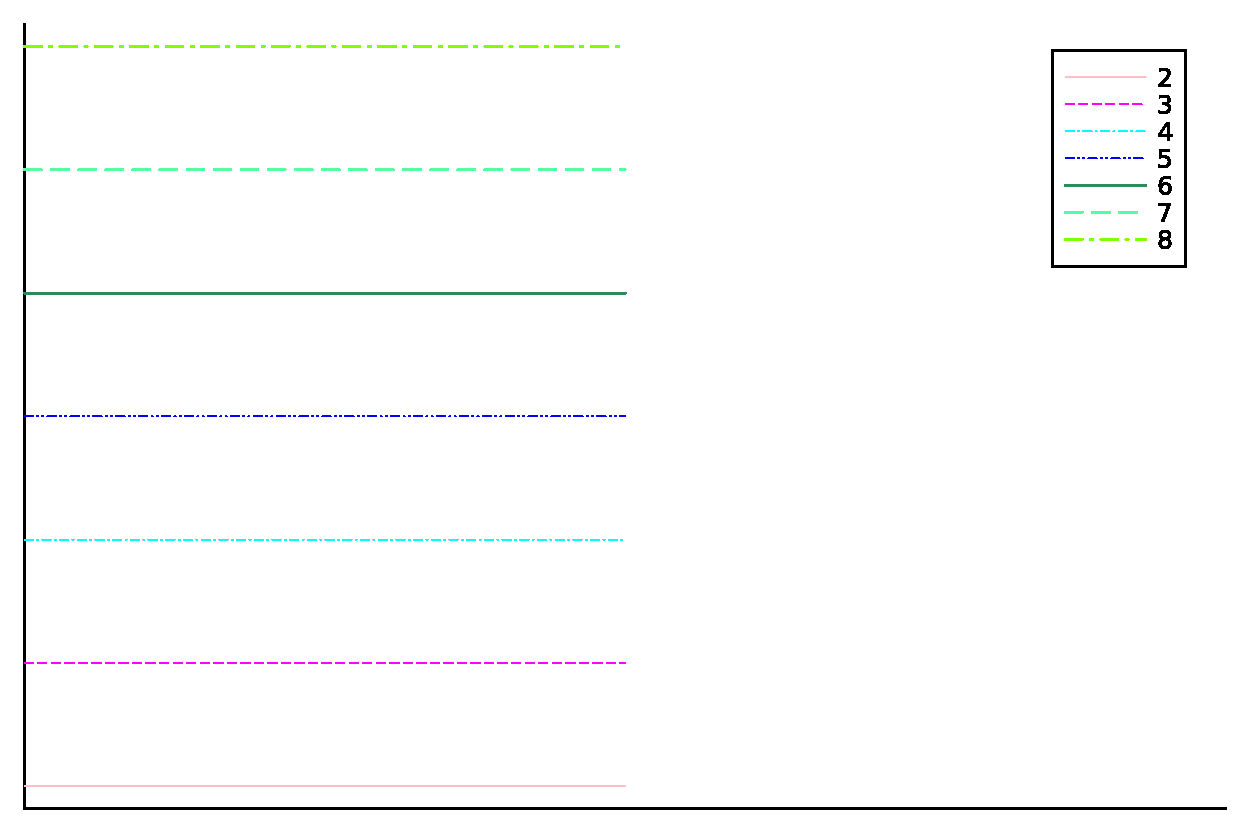
\includegraphics[width=0.08\textwidth, trim={491 180 30 23}, clip]{pdf/odepics/colors_a-d_new_2-8_no_order.pdf}
%	\caption{$\mathcal{D}_1$ Stability Region for IMEX sDeC: orders 2 to 8}
%\label{fig: HundsdorferD1_IMEXsDeC}
%\end{figure}
In Figure~\ref{fig: HundsdorferD1_IMEX} (right), we show the results for the IMEX ADER methods. 
We note that most of the methods fulfill nearly A-stability by almost covering the negative half-plane. %, but most of it except for relatively small, limited sets. 
We highlight that for the equispaced case we do not show the full outreach of the stability regions. 
While in most of the cases, for the almost A-stable cases, these contour lines represent the inner bounds of unlimited stability regions, in the cases of order 5 and 8 we just have large, limited stability regions, as we also could observe for example in the $\mathcal{D}_1$ IMEX DeC case for equispaced nodes. 
Therefore, it seems like we can not guarantee this almost A-stability for the IMEX ADER, but just for some of the orders of accuracy.
%\begin{figure}
%	\centering
%	\begin{minipage}[t]{0.45\textwidth}
%		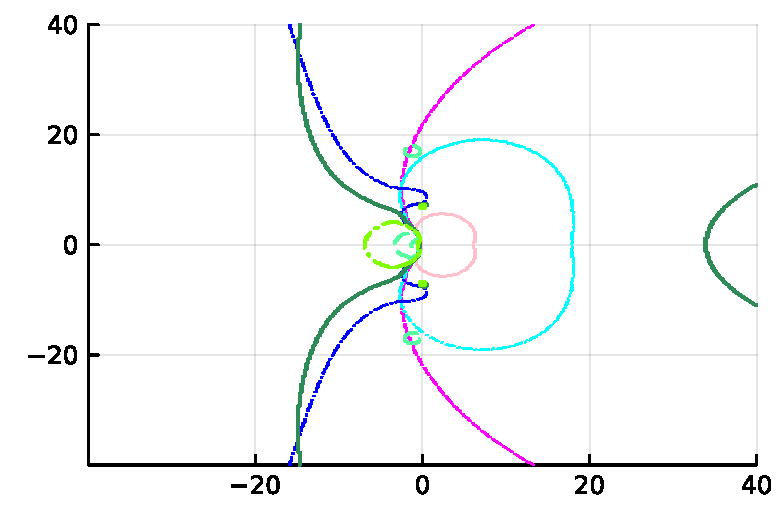
\includegraphics[width=\textwidth]{pdf/odepics/ImExD1_IMEXADER_equispaced_range=40.pdf}
%		\centerline{equispaced nodes}
%	\end{minipage}
%	\begin{minipage}[t]{0.45\textwidth}
%		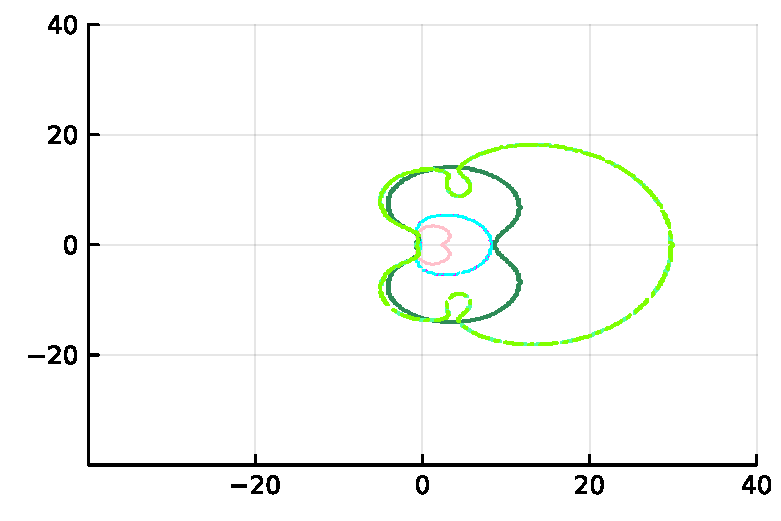
\includegraphics[width=\textwidth]{pdf/odepics/ImExD1_IMEXADER_gaussLobatto_range=40.pdf}
%		\centerline{Gauss-Lobatto nodes}
%	\end{minipage}
%	\includegraphics[width=0.08\textwidth, trim={491 180 30 23}, clip]{pdf/odepics/colors_a-d_new_2-8_no_order.pdf}
%	\caption{$\mathcal{D}_1$ Stability Region for IMEX ADER: orders 2 to 8}
%\label{fig: HundsdorferD1_IMEXADER}
%\end{figure}

%Remark that for the $\mathcal{D}_0$ case, an order of magnitude of the explicit Euler stability region can be considered as good as it gets controlled by the non-stiff term, while for the $\mathcal{D}_1$ case A-stability would be desired due to stiffness. 
Therefore, we can conclude, that some of the IMEX ADER stability regions cover the areas in the complex plane, that we assumed for a stable method in the context of $\mathcal{D}_0$ and $\mathcal{D}_1$, while the DeC and sDeC methods have their limitations with $\mathcal{D}_0= \emptyset$ in every case and bounded stability regions for most of the cases in the scope of $\mathcal{D}_1$. Nevertheless, we need to keep in mind that the set conditions are very strict, so,  the methods might still be applicable to some stiff equations. % \\
These results reflect what we have seen for the respective implicit methods.
\PO{These findings mirror our observations regarding the corresponding implicit methods.} \todo{we may think about deleting equidistant discussion and put the pictures inside the appendix. or shorten this a little bit? Lets discuss}